\documentclass[]{article}
\usepackage{lmodern}
\usepackage{amssymb,amsmath}
\usepackage{ifxetex,ifluatex}
\usepackage{bm}
\usepackage{soul}
\usepackage[color=yellow]{todonotes}
\usepackage{fixltx2e} % provides \textsubscript
\ifnum 0\ifxetex 1\fi\ifluatex 1\fi=0 % if pdftex
  \usepackage[T1]{fontenc}
  \usepackage[utf8]{inputenc}
\else % if luatex or xelatex
  \ifxetex
    \usepackage{mathspec}
  \else
    \usepackage{fontspec}
  \fi
  \defaultfontfeatures{Ligatures=TeX,Scale=MatchLowercase}
\fi
% use upquote if available, for straight quotes in verbatim environments
\IfFileExists{upquote.sty}{\usepackage{upquote}}{}
% use microtype if available
\IfFileExists{microtype.sty}{%
\usepackage{microtype}
\UseMicrotypeSet[protrusion]{basicmath} % disable protrusion for tt fonts
}{}
\usepackage[margin=1in]{geometry}
\usepackage{hyperref}
\hypersetup{unicode=true,
            pdftitle={3 Stationarity, white noise, and some basic time series models},
            pdfauthor={Edward Ionides},
            pdfborder={0 0 0},
            breaklinks=true}
\urlstyle{same}  % don't use monospace font for urls
\usepackage{color}
\usepackage{fancyvrb}
\newcommand{\VerbBar}{|}
\newcommand{\PP}{\mathbb{P}}
\newcommand{\RR}{\mathbb{R}}
\newcommand{\ZZ}{\mathbb{Z}}
\newcommand{\EE}{\mathbb{E}}
\newcommand{\cov}{\text{Cov}}
\newcommand{\VERB}{\Verb[commandchars=\\\{\}]}
\DefineVerbatimEnvironment{Highlighting}{Verbatim}{commandchars=\\\{\}}
% Add ',fontsize=\small' for more characters per line
\usepackage{framed}
\definecolor{shadecolor}{RGB}{248,248,248}
\newenvironment{Shaded}{\begin{snugshade}}{\end{snugshade}}
\newcommand{\KeywordTok}[1]{\textcolor[rgb]{0.13,0.29,0.53}{\textbf{#1}}}
\newcommand{\DataTypeTok}[1]{\textcolor[rgb]{0.13,0.29,0.53}{#1}}
\newcommand{\DecValTok}[1]{\textcolor[rgb]{0.00,0.00,0.81}{#1}}
\newcommand{\BaseNTok}[1]{\textcolor[rgb]{0.00,0.00,0.81}{#1}}
\newcommand{\FloatTok}[1]{\textcolor[rgb]{0.00,0.00,0.81}{#1}}
\newcommand{\ConstantTok}[1]{\textcolor[rgb]{0.00,0.00,0.00}{#1}}
\newcommand{\CharTok}[1]{\textcolor[rgb]{0.31,0.60,0.02}{#1}}
\newcommand{\SpecialCharTok}[1]{\textcolor[rgb]{0.00,0.00,0.00}{#1}}
\newcommand{\StringTok}[1]{\textcolor[rgb]{0.31,0.60,0.02}{#1}}
\newcommand{\VerbatimStringTok}[1]{\textcolor[rgb]{0.31,0.60,0.02}{#1}}
\newcommand{\SpecialStringTok}[1]{\textcolor[rgb]{0.31,0.60,0.02}{#1}}
\newcommand{\ImportTok}[1]{#1}
\newcommand{\CommentTok}[1]{\textcolor[rgb]{0.56,0.35,0.01}{\textit{#1}}}
\newcommand{\DocumentationTok}[1]{\textcolor[rgb]{0.56,0.35,0.01}{\textbf{\textit{#1}}}}
\newcommand{\AnnotationTok}[1]{\textcolor[rgb]{0.56,0.35,0.01}{\textbf{\textit{#1}}}}
\newcommand{\CommentVarTok}[1]{\textcolor[rgb]{0.56,0.35,0.01}{\textbf{\textit{#1}}}}
\newcommand{\OtherTok}[1]{\textcolor[rgb]{0.56,0.35,0.01}{#1}}
\newcommand{\FunctionTok}[1]{\textcolor[rgb]{0.00,0.00,0.00}{#1}}
\newcommand{\VariableTok}[1]{\textcolor[rgb]{0.00,0.00,0.00}{#1}}
\newcommand{\ControlFlowTok}[1]{\textcolor[rgb]{0.13,0.29,0.53}{\textbf{#1}}}
\newcommand{\OperatorTok}[1]{\textcolor[rgb]{0.81,0.36,0.00}{\textbf{#1}}}
\newcommand{\BuiltInTok}[1]{#1}
\newcommand{\ExtensionTok}[1]{#1}
\newcommand{\PreprocessorTok}[1]{\textcolor[rgb]{0.56,0.35,0.01}{\textit{#1}}}
\newcommand{\AttributeTok}[1]{\textcolor[rgb]{0.77,0.63,0.00}{#1}}
\newcommand{\RegionMarkerTok}[1]{#1}
\newcommand{\InformationTok}[1]{\textcolor[rgb]{0.56,0.35,0.01}{\textbf{\textit{#1}}}}
\newcommand{\WarningTok}[1]{\textcolor[rgb]{0.56,0.35,0.01}{\textbf{\textit{#1}}}}
\newcommand{\AlertTok}[1]{\textcolor[rgb]{0.94,0.16,0.16}{#1}}
\newcommand{\ErrorTok}[1]{\textcolor[rgb]{0.64,0.00,0.00}{\textbf{#1}}}
\newcommand{\NormalTok}[1]{#1}
\usepackage{graphicx,grffile}
\makeatletter
\def\maxwidth{\ifdim\Gin@nat@width>\linewidth\linewidth\else\Gin@nat@width\fi}
\def\maxheight{\ifdim\Gin@nat@height>\textheight\textheight\else\Gin@nat@height\fi}
\makeatother
% Scale images if necessary, so that they will not overflow the page
% margins by default, and it is still possible to overwrite the defaults
% using explicit options in \includegraphics[width, height, ...]{}
\setkeys{Gin}{width=\maxwidth,height=\maxheight,keepaspectratio}
\IfFileExists{parskip.sty}{%
\usepackage{parskip}
}{% else
\setlength{\parindent}{0pt}
\setlength{\parskip}{6pt plus 2pt minus 1pt}
}
\setlength{\emergencystretch}{3em}  % prevent overfull lines
\providecommand{\tightlist}{%
  \setlength{\itemsep}{0pt}\setlength{\parskip}{0pt}}
%\setcounter{secnumdepth}{0}
\setcounter{section}{3}
% Redefines (sub)paragraphs to behave more like sections
\ifx\paragraph\undefined\else
\let\oldparagraph\paragraph
\renewcommand{\paragraph}[1]{\oldparagraph{#1}\mbox{}}
\fi
\ifx\subparagraph\undefined\else
\let\oldsubparagraph\subparagraph
\renewcommand{\subparagraph}[1]{\oldsubparagraph{#1}\mbox{}}
\fi

%%% Use protect on footnotes to avoid problems with footnotes in titles
\let\rmarkdownfootnote\footnote%
\def\footnote{\protect\rmarkdownfootnote}

%%% Change title format to be more compact
\usepackage{titling}

% Create subtitle command for use in maketitle
\newcommand{\subtitle}[1]{
  \posttitle{
    \begin{center}\large#1\end{center}
    }
}

\setlength{\droptitle}{-2em}
  \title{3. Stationarity, white noise, and some basic time series models}
  \pretitle{\vspace{\droptitle}\centering\huge}
  \posttitle{\par}
  \author{Edward Ionides}
  \preauthor{\centering\large\emph}
  \postauthor{\par}
  \predate{\centering\large\emph}
  \postdate{\par}
  \date{1/9/2018}


\begin{document}
\maketitle

{
\setcounter{tocdepth}{2}
\tableofcontents
}
\newcommand\prob{\mathbb{P}}
\newcommand\E{\mathbb{E}}
\newcommand\var{\mathrm{Var}}
\newcommand\loglik{\ell}
\newcommand\R{\mathbb{R}}
\newcommand\data[1]{#1^*}
\newcommand\given{\, ; \,}
\newcommand\transpose{\scriptsize{T}}





\begin{center}\rule{0.5\linewidth}{\linethickness}\end{center}

\begin{center}\rule{0.5\linewidth}{\linethickness}\end{center}

Objectives

\begin{enumerate}
\def\labelenumi{\arabic{enumi}.}
\item
  Define different concepts for stationarity.
\item
  Define white noise.
\item
  Use white noise to construct some basic time series models.
\end{enumerate}

\begin{center}\rule{0.5\linewidth}{\linethickness}\end{center}

\begin{center}\rule{0.5\linewidth}{\linethickness}\end{center}

\subsection{Definition: Weak stationarity and strict
stationarity}\label{definition-weak-stationarity-and-strict-stationarity}

\begin{itemize}
\item
  A time series model which is both mean stationary and covariance
  stationary is called \hl{\textbf{weakly stationary}.}
  \todo[inline]{Typically we call ``weakly stationary'' just ``stationary'', and say ``strictly stationary'' otherwise.}
\item
  A time series model for which all joint distributions are invariant to
  shifts in time is called \hl{\textbf{strictly stationary}}.

  \begin{itemize}
  \item
    Formally, this means that for any collection of times
    \((t_1, t_2,\dots,t_K)\), the joint distribution of observations at
    these times should be the same as the joint distribution at
    \((t_1+\tau, t_2+\tau,\dots,t_K+\tau)\) for any \(\tau\).
  \item
    For equally spaced observations, this becomes: for any collection of
    timepoints \(n_1,\dots,n_K\), and for any lag \(h\), the joint
    density function of \((Y_{n_1},Y_{n_2},\dots, Y_{n_K})\) is the same
    as the joint density function of
    \((Y_{n_1+h},Y_{n_2+h},\dots, Y_{n_K+h})\).
  \item
    In our general notation for densities, this strict stationarity
    requirement can be written as

    \begin{eqnarray}&&f_{Y_{n_1},Y_{n_2},\dots, Y_{n_K}}(y_1,y_2,\dots,y_K)\\
    &&\quad\quad = f_{Y_{n_1+h},Y_{n_2+h},\dots, Y_{n_K+h}}(y_1,y_2,\dots,y_K).
    \end{eqnarray}
  \end{itemize}
\item
  Strict stationarity implies weak stationarity (check this). Note that
  we only defined weak stationarity for equally spaced observations.
\end{itemize}

\begin{center}\rule{0.5\linewidth}{\linethickness}\end{center}

\begin{center}\rule{0.5\linewidth}{\linethickness}\end{center}

\subsubsection{Question: How could we assess whether a weak stationary
model is appropriate for a time series
dataset?}\label{question-how-could-we-assess-whether-a-weak-stationary-model-is-appropriate-for-a-time-series-dataset}

\todo[inline]{Suppose observations are equally spaced scross time. Can calculate averages in chunks (i.e. time windows) for mean-stationary. Can calculate sample ACF in time windows. Perhaps the sample ACF decays quickly to zero, that would support \textbf{weakly stationary}, since a trend typically shows up as a \textbf{long range} pattern in the sample ACF.}

\begin{center}\rule{0.5\linewidth}{\linethickness}\end{center}

\begin{center}\rule{0.5\linewidth}{\linethickness}\end{center}

\subsubsection{Question: How could we assess whether a strictly
stationary model is appropriate for a time series
dataset?}\label{question-how-could-we-assess-whether-a-strictly-stationary-model-is-appropriate-for-a-time-series-dataset}

\todo[inline]{We essentially can't.}

\begin{center}\rule{0.5\linewidth}{\linethickness}\end{center}

\begin{center}\rule{0.5\linewidth}{\linethickness}\end{center}

\subsubsection{Question: Is it usual for time series to be well modeled
as stationary (either weakly or
strictly)?}\label{question-is-it-usual-for-time-series-to-be-well-modeled-as-stationary-either-weakly-or-strictly}

ANSWER: It sometimes happens. However, systems often change over time,
and that may be one of the things we are interested in.

\begin{center}\rule{0.5\linewidth}{\linethickness}\end{center}

\begin{center}\rule{0.5\linewidth}{\linethickness}\end{center}

\subsubsection{Question: If data do not often show stationary behavior,
why do many fundamental models have
stationarity?}\label{question-if-data-do-not-often-show-stationary-behavior-why-do-many-fundamental-models-have-stationarity}

\todo[inline]{Stationary models are building blocks for non-stationary models.}

\begin{center}\rule{0.5\linewidth}{\linethickness}\end{center}

\begin{center}\rule{0.5\linewidth}{\linethickness}\end{center}

\subsubsection{Question: Is a stationary model appropriate for either
(or both) the time series below?
Explain.}\label{question-is-a-stationary-model-appropriate-for-either-or-both-the-time-series-below-explain.}

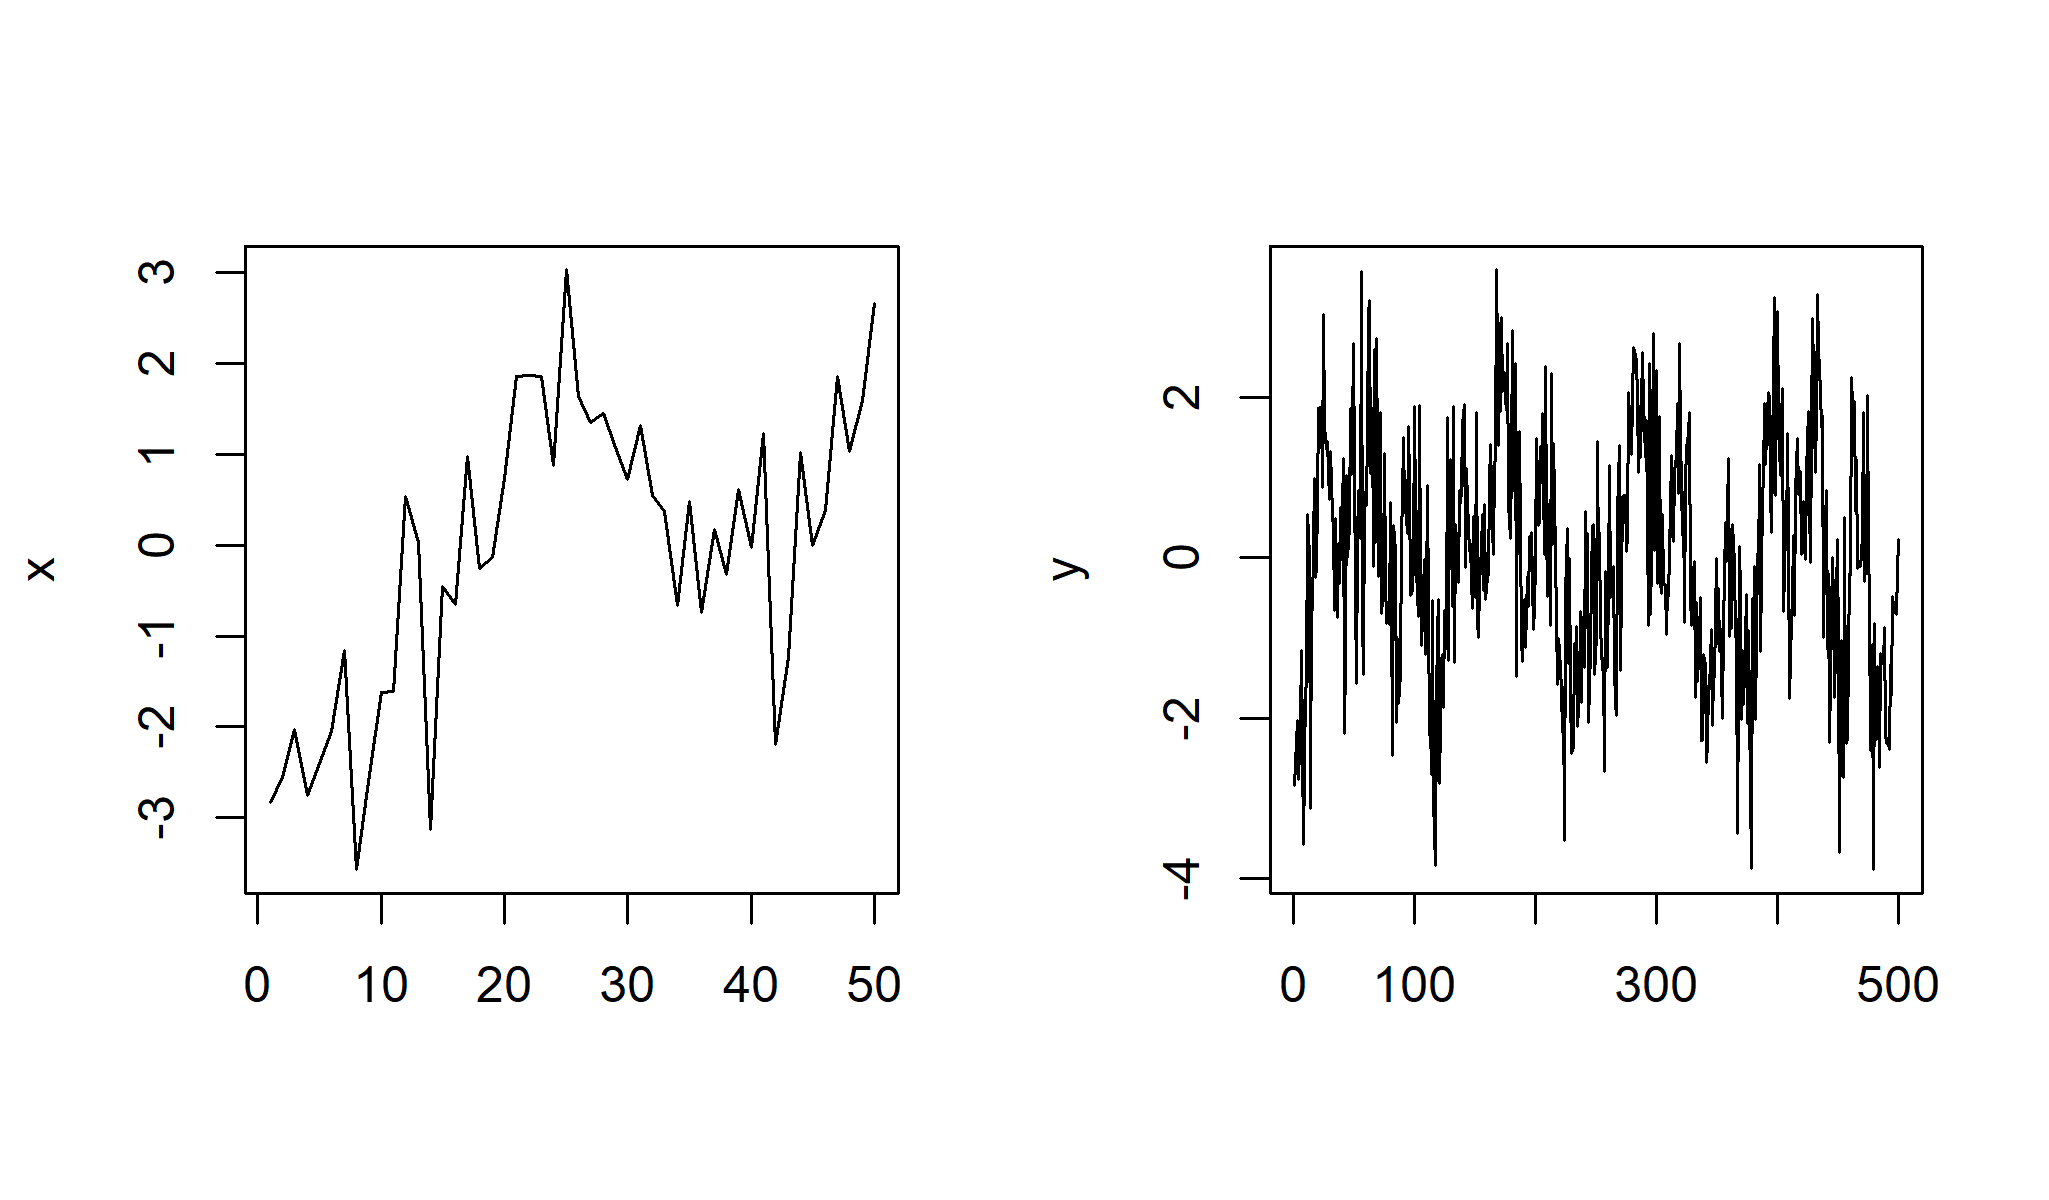
\includegraphics{figure/intro-stationarity_sim-1.png}

\todo[inline]{Here, $X = Y[1:50]$, so we really need the entire data set to be able to assess stationarity.}

\begin{center}\rule{0.5\linewidth}{\linethickness}\end{center}

\begin{center}\rule{0.5\linewidth}{\linethickness}\end{center}

\subsection{White noise}\label{white-noise}

A time series model \(\epsilon_{1:N}\) which is weakly stationary with

\begin{eqnarray}
\E[\epsilon_n]&=& 0 \\
\cov(\epsilon_m,\epsilon_n) &=& \left\{\begin{array}{ll}
  \sigma^2, & \mbox{if $m=n$} \\
   0, & \mbox{if $m\neq n$} \end{array}\right. ,
\end{eqnarray}

is said to be \textbf{white noise} with variance \(\sigma^2\).

\begin{itemize}
\item
  The ``noise'' is because there's no pattern, just random variation. If
  you listened to a realization of white noise as an audio file, you
  would hear a static sound.
\item
  The ``white'' is because all freqencies are equally represented. This
  will become clear when we do frequency domain analysis of time series.
\item
  Signal processing---sending and receiving signals on noisy
  channels---was a motivation for early time series analysis.
\end{itemize}

\begin{center}\rule{0.5\linewidth}{\linethickness}\end{center}

\begin{center}\rule{0.5\linewidth}{\linethickness}\end{center}

\subsubsection{Example: Gaussian white
noise}\label{example-gaussian-white-noise}

In time series analysis, a sequence of independent identically
distributed (IID) Normal random variables with mean zero and variance
\(\sigma^2\) is known as \textbf{Gaussian white noise}. We write this
model as \[ \epsilon_{1:N} \sim \mbox{IID } N[0,\sigma^2].\]

\begin{center}\rule{0.5\linewidth}{\linethickness}\end{center}

\begin{center}\rule{0.5\linewidth}{\linethickness}\end{center}

\subsubsection{Example: Binary white
noise}\label{example-binary-white-noise}

Let \(\epsilon_{1:N}\) be IID with

\begin{eqnarray}
\epsilon_n = \left\{\begin{array}{ll}
  1, & \mbox{with probability $1/2$} \\
  -1, & \mbox{with probability $1/2$} \end{array}\right. .
\end{eqnarray}

We can check that \(\E[\epsilon_n]=0\), \(\var(\epsilon_n)=1\) and
\(\cov(\epsilon_m,\epsilon_n)=0\) for \(m\neq n\). Therefore,
\(\epsilon_{1:N}\) is white noise.

Similarly, for any \(p\in (0,1)\), we could have

\begin{eqnarray}
\epsilon_n = \left\{\begin{array}{ll}
  (1-p)/p, & \mbox{with probability $p$} \\
  -1, & \mbox{with probability $1-p$} \end{array}\right. .
\end{eqnarray}

\begin{center}\rule{0.5\linewidth}{\linethickness}\end{center}

\begin{center}\rule{0.5\linewidth}{\linethickness}\end{center}

\subsubsection{Example: Sinusoidal white
noise}\label{example-sinusoidal-white-noise}

Let \(\epsilon_n = \sin(2\pi n U)\), with a single draw
\(U\sim\mathrm{Uniform}[0,1]\) determining the time series model for all
\(n\in 1:N\).

\textbf{A}. Show that \(\epsilon_{1:N}\) is weakly stationary, and is
white noise!

\hl{\textbf{ANS.}} We have $\EE(\epsilon_n) = \int_{0}^{1}\sin(2\pi nu)\,du=\left[-\frac{1}{2\pi n}\cos(2\pi n u)\right]^1_0 = 0$. Then, for $m\neq n$,
\begin{align*}
\cov(\epsilon_m,\epsilon_n) = \EE(\epsilon_m\epsilon_n) &= \int_{0}^{1}\sin(2\pi mu)\sin(2\pi n u)\, du\\
&=\frac{1}{2}\int_{0}^{1}\cos(2\pi(m-n)u) - \cos(2\pi(m+n)u)\, du\\
&=0.
\end{align*}
Now, for $m=n$,
$$\cov(\epsilon_m,\epsilon_n) = \int_{0}^{1}\sin^2(2\pi nu)\, du=\frac{1}{2}\int_{0}^{1}\left[1-\cos(4\pi nu)\right]\, du = \frac{1}{2}. $$

\textbf{B}. Show that \(\epsilon_{1:N}\) is NOT strictly stationary.

\hl{\textbf{ANS.}} We have $\PP(\epsilon_1 > 1-\delta,\, \epsilon_2\in[-\delta,
\delta])>0$ but $\PP(\epsilon_2>1-\delta,\, \epsilon_3\in [-\delta,\delta])=0$. Thus, the model is not invariant to time lags.

\begin{itemize}
\item
  These are exercises in working with sines and cosines.
\item
  As well as providing a concrete example of a weakly stationary time
  series that is not strictly stationary, practice working with sines
  and cosines will come in handy later when we work in the frequency
  domain.
\item
  As a hint for B, consider the following plot of \(\epsilon_{1:3}\) as
  a function of \(U\). \(\epsilon_1\) is shown as the black solid line;
  \(\epsilon_2\) is the red dashed line; \(\epsilon_3\) is the blue
  dot-dash line.
\end{itemize}

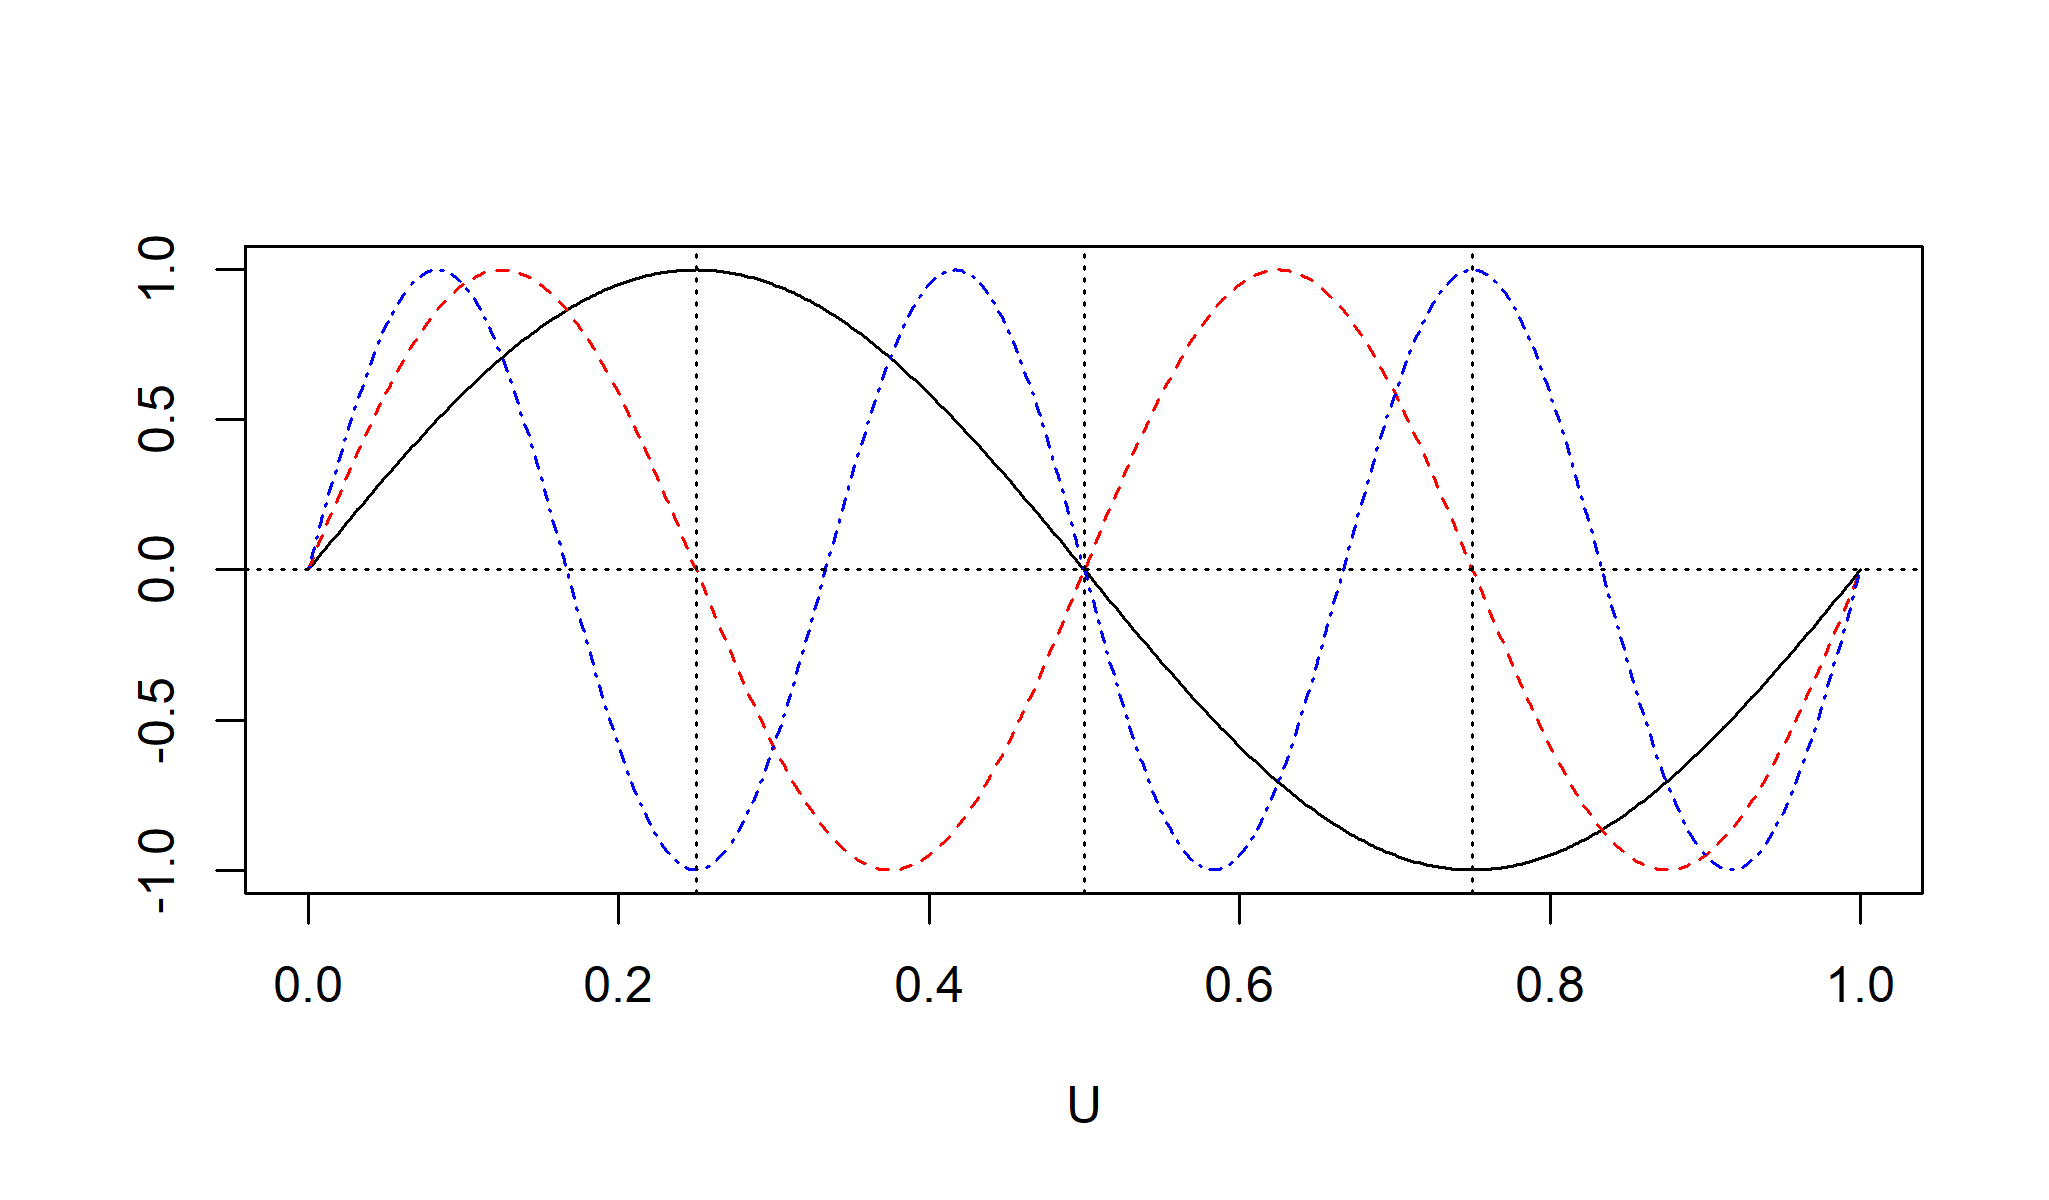
\includegraphics{figure/intro-sinusoidal-1.png}

\begin{itemize}
\tightlist
\item
  Now we're going to use white noise as a building block for various
  other time series models.
\end{itemize}

\begin{center}\rule{0.5\linewidth}{\linethickness}\end{center}

\begin{center}\rule{0.5\linewidth}{\linethickness}\end{center}

\subsubsection{Reminder: why do we need time series
models?}\label{reminder-why-do-we-need-time-series-models}

\begin{itemize}
\item
  All statistical tests (i.e., whenever we use data to answer a
  question) rely on having a model for the data. The model is sometimes
  called the \textbf{assumptions} for the test.
\item
  If our model is wrong, then any conclusions drawn from it may be
  wrong. Our error could be small and insignificant, or disastrous.
\item
  Time series data collected close in time are often more similar than a
  model with IID variation would predict. We need models that have this
  property, and we must work out how to test interesting hypotheses for
  these models.
\end{itemize}

\begin{center}\rule{0.5\linewidth}{\linethickness}\end{center}

\begin{center}\rule{0.5\linewidth}{\linethickness}\end{center}

\subsection{Autoregressive models}\label{autoregressive-models}

\subsubsection{The AR(p) autoregressive
model}\label{the-arp-autoregressive-model}

\begin{itemize}
\item
  The order \(p\) autoregressive model, abbreviated to AR(p), is
  $${[}M1{]}
  \quad\quad \quad Y_n = \phi_1 Y_{n-1}+\phi_2Y_{n-2}+\dots+\phi_pY_{n-p} + \epsilon_n,$$
  where \(\{\epsilon_n\}\) is a white noise process.
\item
  Often, we consider the \textbf{Gaussian AR(p)} model, where
  \(\{\epsilon_n\}\) is a Gaussian white noise process.
\item
  M1 is a \textbf{stochastic difference equation}. It is a
  \href{https://en.wikipedia.org/wiki/Recurrence_relation}{difference
  equation (also known as a recurrence relation)} since \hl{each time point
  is specified recursively in terms of previous time points. Stochastic
  just means random.}
\item
  To complete the model, we need to \textbf{initialize} the solution to
  the stochastic difference equation. Supposing we want to specify a
  distribution for \(Y_{1:N}\), we have some choices in how to set up
  the \textbf{initial values}.

  \begin{enumerate}
  \def\labelenumi{\arabic{enumi}.}
  \item
    We can specify \(Y_{1:p}\) explicitly, to get the recursion started.
  \item
    We can specify \(Y_{1-p:0}\) explicitly.
  \item
    For either of these choices, we can define these initial values
    either to be additional parameters in the model (i.e., not random)
    or to be specified random variables.
  \item
    If we want our model is strictly stationary, we must initialize so
    that \(Y_{1:p}\) have the proper joint distribution for this
    stationary model.
  \end{enumerate}
\item
  Let's investigate a particular Gaussian AR(1) process, as an exercise.
  $${[}M2{]} \quad\quad \quad Y_n = 0.6 Y_{n-1}+ \epsilon_n,$$ where
  \(\epsilon_n\sim \mathrm{IID} N[0,1]\). We will initialize with
  \(Y_1\sim N[0,1.56^2]\).
\end{itemize}

\begin{center}\rule{0.5\linewidth}{\linethickness}\end{center}

\begin{center}\rule{0.5\linewidth}{\linethickness}\end{center}

\subsubsection{Simulating an autoregressive
model}\label{simulating-an-autoregressive-model}

\begin{itemize}
\item
  Looking at simulated sample paths is a good way to get some intuition
  about a random process model.
\item
  We will do this for the AR(1) model M2
\item
  One approach is to use the \texttt{arima.sim} function in R.
\end{itemize}

\begin{Shaded}
\begin{Highlighting}[]
\KeywordTok{set.seed}\NormalTok{(}\DecValTok{123456789}\NormalTok{)}
\NormalTok{ar1 <-}\StringTok{ }\KeywordTok{arima.sim}\NormalTok{(}\KeywordTok{list}\NormalTok{(}\DataTypeTok{ar=}\FloatTok{0.6}\NormalTok{),}\DataTypeTok{n=}\DecValTok{100}\NormalTok{,}\DataTypeTok{sd=}\DecValTok{1}\NormalTok{)}
\KeywordTok{plot}\NormalTok{(ar1,}\DataTypeTok{type=}\StringTok{"l"}\NormalTok{)}
\end{Highlighting}
\end{Shaded}

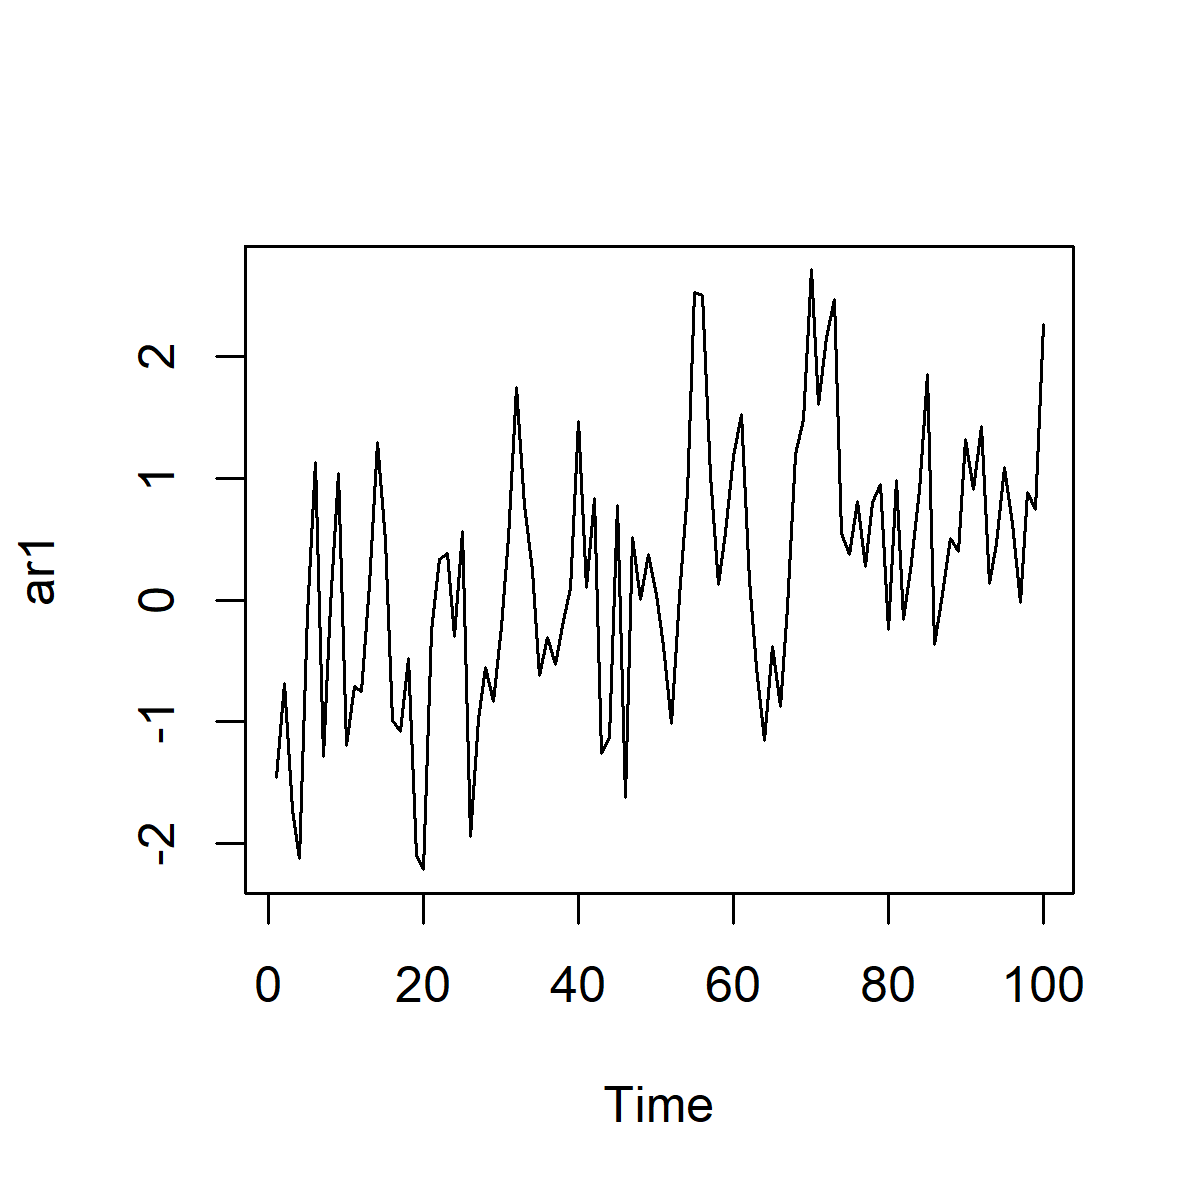
\includegraphics{figure/intro-ar_arima_sim-1.png}

\begin{itemize}
\item
  Does your intuition tell you that these \hl{data are evidence for a model
  with a linear trend?}
\item
  The eye looks for patterns in data, and often finds them even when
  there is no strong statistical evidence.
\item
  That is why we need statistical tests!
\item
  It is easy to see patterns even in white noise. Dependent models
  produce spurious patterns even more often.
\item
  Play with simulating different models with different seeds to train
  your intuition.
\item
  A direct approach to simulating model M2 is to write out the model
  equation explicitly.
\end{itemize}

\begin{Shaded}
\begin{Highlighting}[]
\KeywordTok{set.seed}\NormalTok{(}\DecValTok{123456789}\NormalTok{)}
\NormalTok{N <-}\StringTok{ }\DecValTok{100}
\NormalTok{X <-}\StringTok{ }\KeywordTok{numeric}\NormalTok{(N)}
\NormalTok{X[}\DecValTok{1}\NormalTok{] <-}\StringTok{ }\KeywordTok{rnorm}\NormalTok{(}\DecValTok{1}\NormalTok{,}\DataTypeTok{sd=}\FloatTok{1.56}\NormalTok{)}
\ControlFlowTok{for}\NormalTok{(n }\ControlFlowTok{in} \DecValTok{2}\OperatorTok{:}\NormalTok{N) X[n] <-}\StringTok{ }\FloatTok{0.6} \OperatorTok{*}\StringTok{ }\NormalTok{X[n}\OperatorTok{-}\DecValTok{1}\NormalTok{] }\OperatorTok{+}\StringTok{ }\KeywordTok{rnorm}\NormalTok{(}\DecValTok{1}\NormalTok{)}
\KeywordTok{plot}\NormalTok{(X,}\DataTypeTok{type=}\StringTok{"l"}\NormalTok{)}
\end{Highlighting}
\end{Shaded}

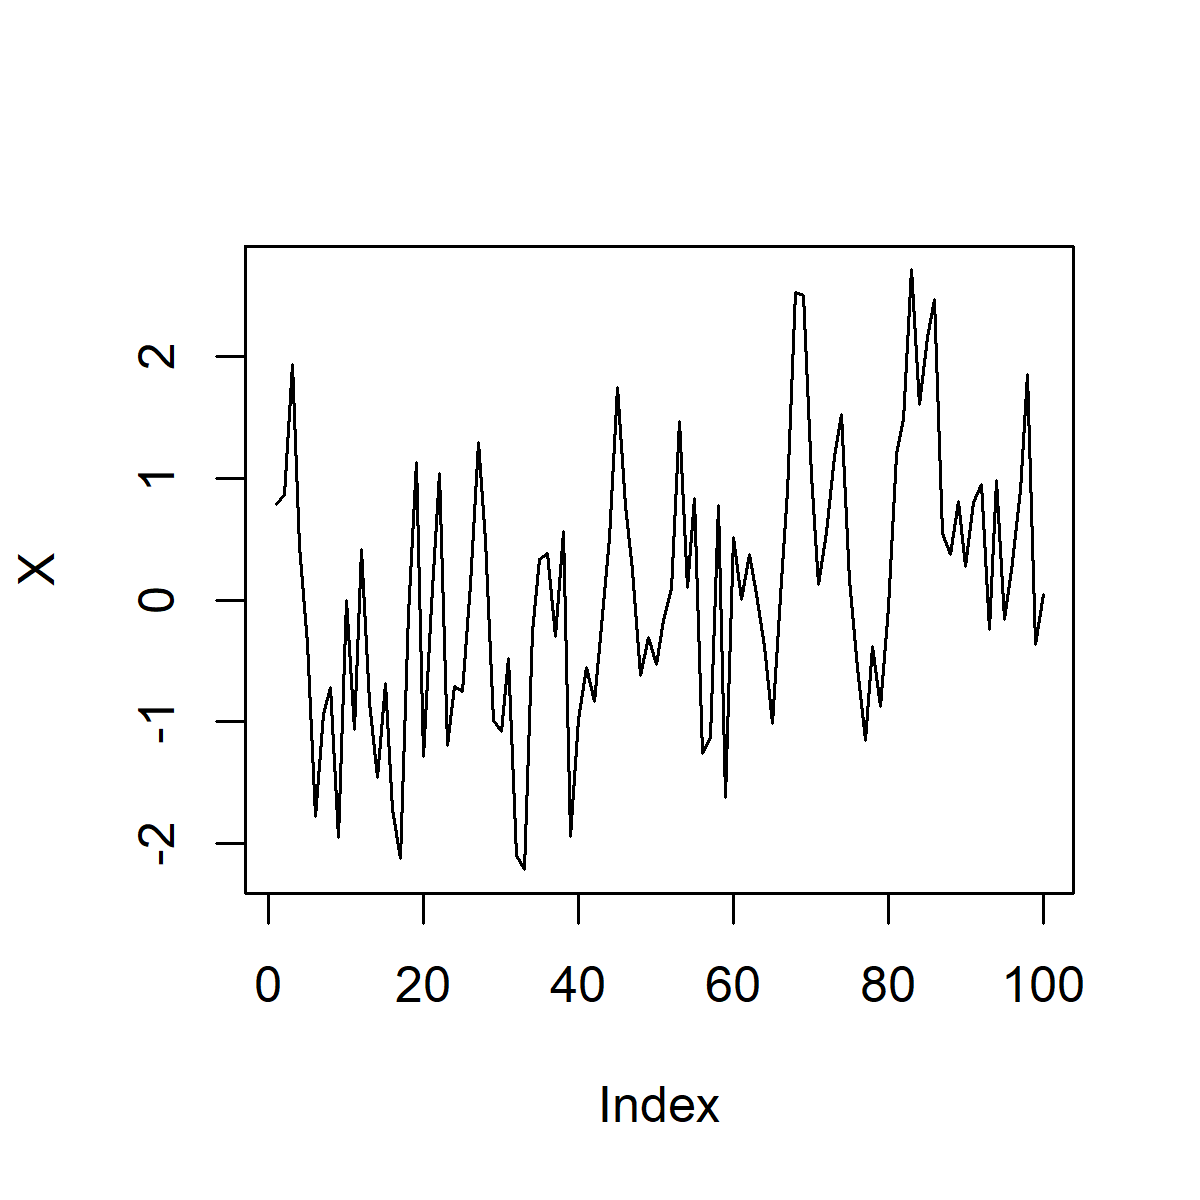
\includegraphics{figure/intro-ar_sim-1.png}

\begin{itemize}
\tightlist
\item
  This looks very similar to the \texttt{arima.sim} simulation, except
  for a difference near the start. Can you explain this? Hint: How does
  \texttt{arima.sim} initialize the simulation?
\end{itemize}

\begin{center}\rule{0.5\linewidth}{\linethickness}\end{center}

\begin{center}\rule{0.5\linewidth}{\linethickness}\end{center}

\subsubsection{\texorpdfstring{What are the advantages and disadvantages
of \texttt{arima.sim} over the direct simulation
method?}{What are the advantages and disadvantages of arima.sim over the direct simulation method?}}\label{what-are-the-advantages-and-disadvantages-of-arima.sim-over-the-direct-simulation-method}

\begin{center}\rule{0.5\linewidth}{\linethickness}\end{center}

\begin{center}\rule{0.5\linewidth}{\linethickness}\end{center}

\subsubsection{Exercise: Compute the autcovariance function for model
M2.}\label{exercise-compute-the-autcovariance-function-for-model-m2.}

\begin{center}\rule{0.5\linewidth}{\linethickness}\end{center}

\begin{center}\rule{0.5\linewidth}{\linethickness}\end{center}

\subsection{Moving average models}\label{moving-average-models}

\subsubsection{The MA(q) moving average
model}\label{the-maq-moving-average-model}

\begin{itemize}
\item
  The \hl{order $q$ moving average model}, abbreviated to MA(q), is
  $${[}M3{]}
  \quad\quad \quad Y_n = \epsilon_n +\theta_1 \epsilon_{n-1} +\dots+\theta_q\epsilon_{n-q},$$
  where \(\{\epsilon_n\}\) is a white noise process.
  \todo[inline]{Moving average models are always stationary.}
\item
  To fully specify \(Y_{1:N}\) we must specify the joint distribution of
  \(\epsilon_{1-q:N}\).
\item
  Often, we consider the \hl{\textbf{Gaussian MA(q)} model, where
  $\epsilon_n$ is a Gaussian white noise process.}
\item
  Let's investigate a particular Gaussian MA(2) process, as an exercise.
  $${[}M4{]}
  \quad\quad \quad Y_n = \epsilon_n + 1.5\epsilon_{n-1}+\epsilon_{n-2},$$
  where \(\epsilon_n\sim \mathrm{IID} N[0,1]\).
\end{itemize}

\subsubsection{Simulating a moving average
model}\label{simulating-a-moving-average-model}

\begin{itemize}
\tightlist
\item
  Let's simulate M4 using both the methods we tried for the
  autoregressive model
\end{itemize}

\begin{Shaded}
\begin{Highlighting}[]
\NormalTok{N <-}\StringTok{ }\DecValTok{100}
\KeywordTok{set.seed}\NormalTok{(}\DecValTok{123456789}\NormalTok{)}
\NormalTok{X1 <-}\StringTok{ }\KeywordTok{arima.sim}\NormalTok{(}\KeywordTok{list}\NormalTok{(}\DataTypeTok{ma=}\KeywordTok{c}\NormalTok{(}\FloatTok{1.5}\NormalTok{,}\DecValTok{1}\NormalTok{)),}\DataTypeTok{n=}\NormalTok{N,}\DataTypeTok{sd=}\DecValTok{1}\NormalTok{)}
\KeywordTok{set.seed}\NormalTok{(}\DecValTok{123456789}\NormalTok{)}
\NormalTok{epsilon <-}\StringTok{ }\KeywordTok{rnorm}\NormalTok{(N}\OperatorTok{+}\DecValTok{2}\NormalTok{)}
\NormalTok{X2 <-}\StringTok{ }\KeywordTok{numeric}\NormalTok{(N)}
\ControlFlowTok{for}\NormalTok{(n }\ControlFlowTok{in} \DecValTok{1}\OperatorTok{:}\NormalTok{N) X2[n] <-}\StringTok{ }\NormalTok{epsilon[n}\OperatorTok{+}\DecValTok{2}\NormalTok{]}\OperatorTok{+}\FloatTok{1.5}\OperatorTok{*}\NormalTok{epsilon[n}\OperatorTok{+}\DecValTok{1}\NormalTok{]}\OperatorTok{+}\NormalTok{epsilon[n]}
\NormalTok{oldpars <-}\StringTok{ }\KeywordTok{par}\NormalTok{(}\DataTypeTok{mfrow=}\KeywordTok{c}\NormalTok{(}\DecValTok{1}\NormalTok{,}\DecValTok{2}\NormalTok{))}
\KeywordTok{plot}\NormalTok{(X1,}\DataTypeTok{type=}\StringTok{"l"}\NormalTok{)}
\KeywordTok{plot}\NormalTok{(X2,}\DataTypeTok{type=}\StringTok{"l"}\NormalTok{)}
\end{Highlighting}
\end{Shaded}
\todo[inline]{Argument 'ma=' as upposed to 'ar=' when we simulate the AR(1) model.}
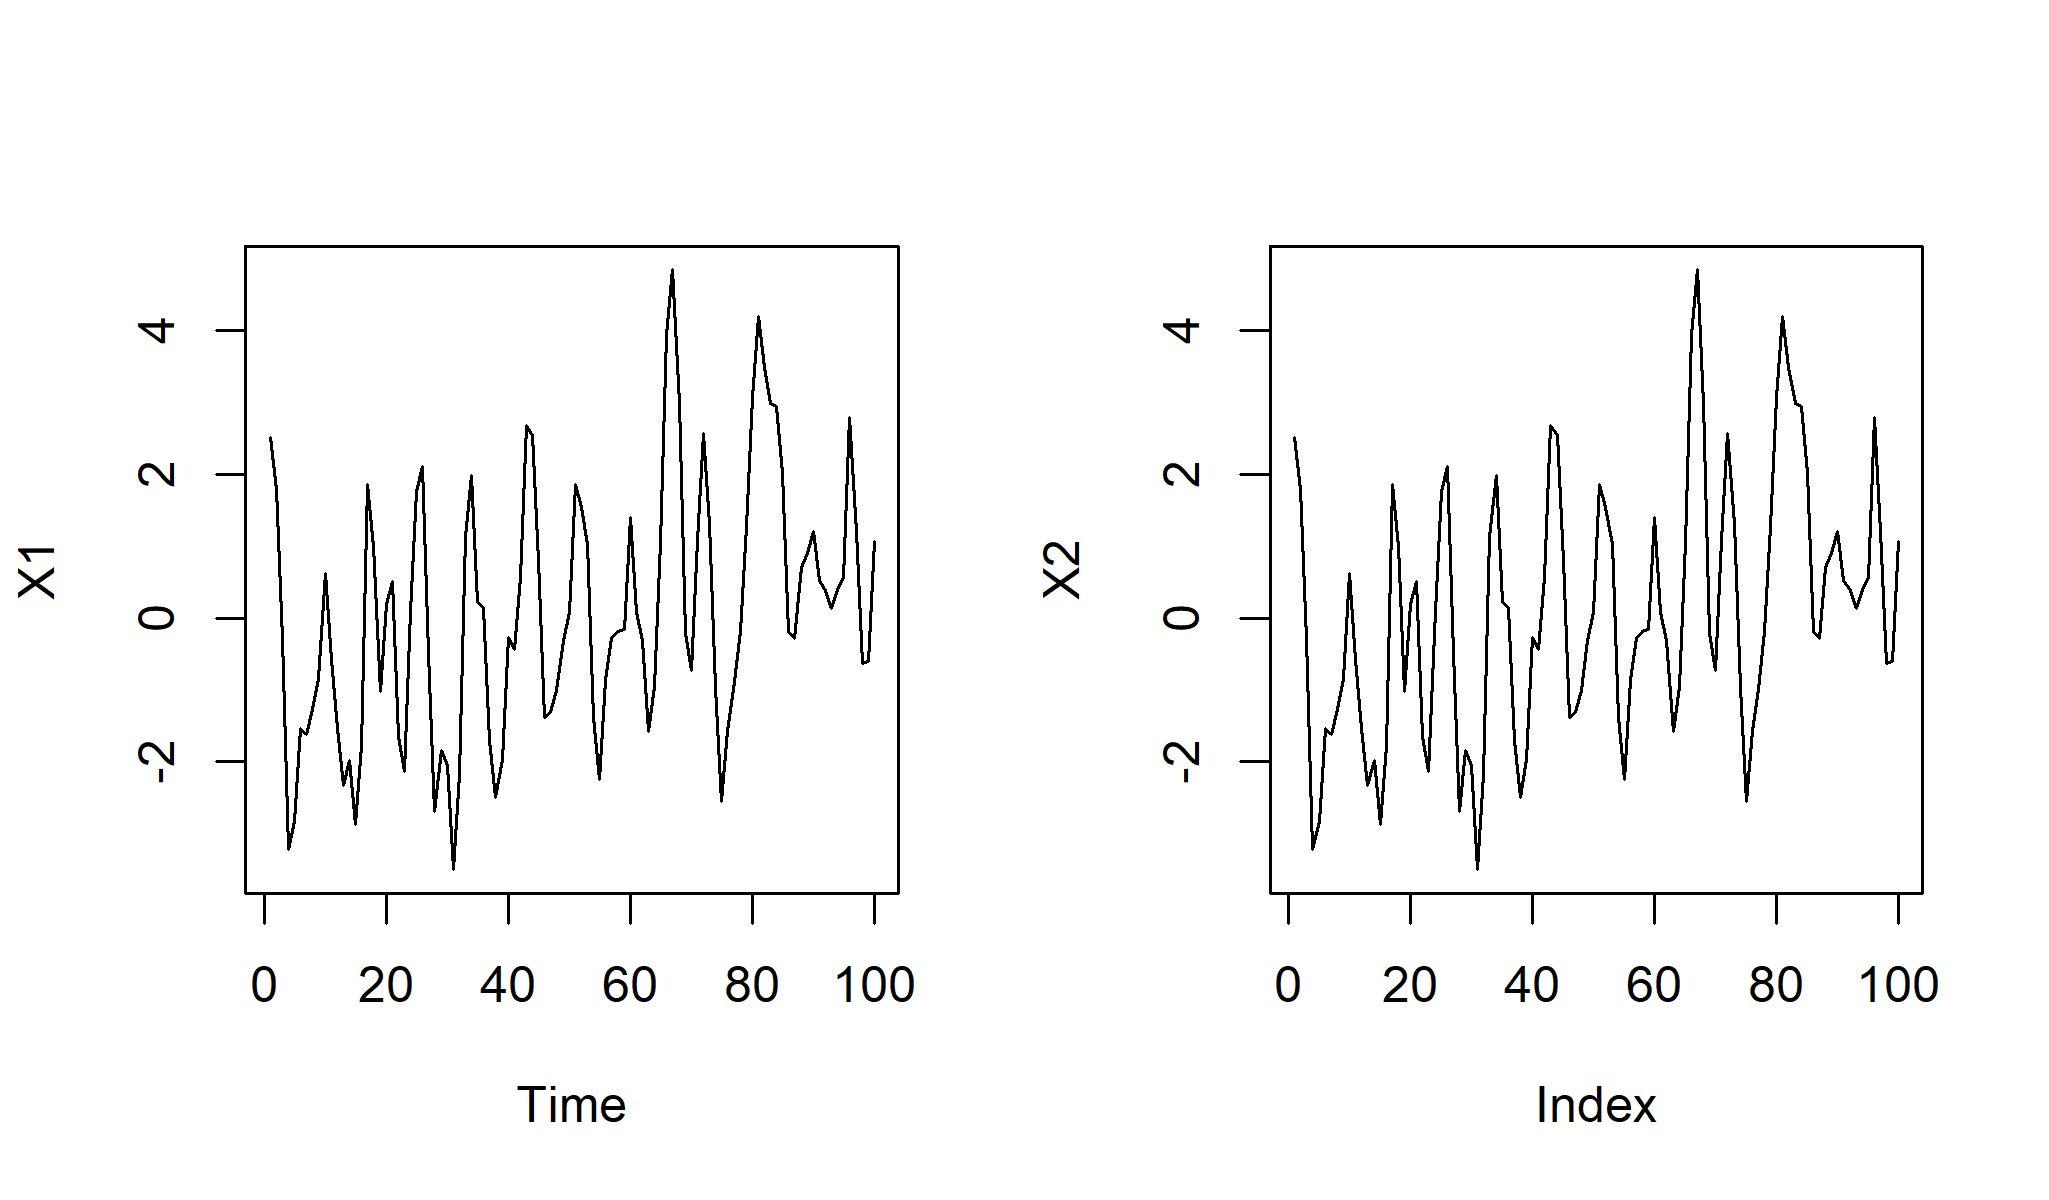
\includegraphics{figure/intro-ma_sim-1.png}

\begin{Shaded}
\begin{Highlighting}[]
\KeywordTok{par}\NormalTok{(oldpars)}
\end{Highlighting}
\end{Shaded}

\begin{itemize}
\tightlist
\item
  \texttt{X1} and \texttt{X2} look identical. We can check this
\end{itemize}

\begin{Shaded}
\begin{Highlighting}[]
\KeywordTok{all}\NormalTok{(X1}\OperatorTok{==}\NormalTok{X2)}
\end{Highlighting}
\end{Shaded}

\begin{verbatim}
## [1] TRUE
\end{verbatim}

\begin{itemize}
\item
  Perhaps you agree that the spurious evidence for a trend that we saw
  for the AR(1) model is still somewhat present for the MA(2)
  simulation.
\item
  We could be curious about what the underlying white noise process
  looks like
\end{itemize}

\begin{Shaded}
\begin{Highlighting}[]
\NormalTok{N <-}\StringTok{ }\DecValTok{100}
\KeywordTok{set.seed}\NormalTok{(}\DecValTok{123456789}\NormalTok{)}
\NormalTok{epsilon <-}\StringTok{ }\KeywordTok{rnorm}\NormalTok{(N)}
\KeywordTok{plot}\NormalTok{(epsilon,}\DataTypeTok{type=}\StringTok{"l"}\NormalTok{)}
\end{Highlighting}
\end{Shaded}

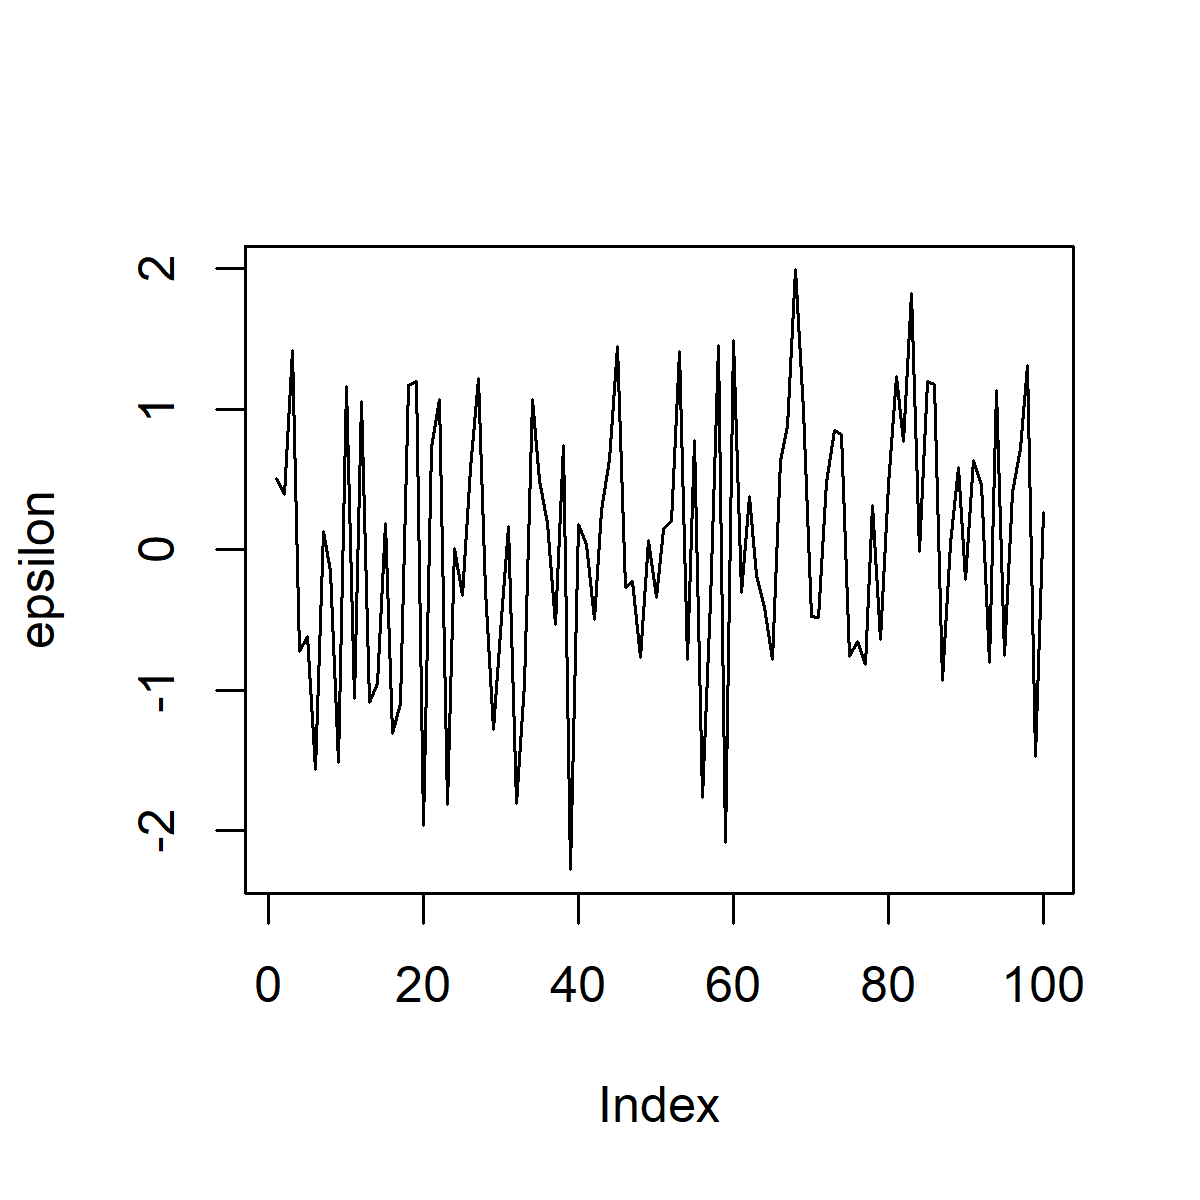
\includegraphics{figure/intro-noise_sim-1.png}

\begin{itemize}
\tightlist
\item
  To me, the trend-like behavior is not visually apparent in the white
  noise that ``drives'' the AR and MA models.
\end{itemize}

\begin{center}\rule{0.5\linewidth}{\linethickness}\end{center}

\begin{center}\rule{0.5\linewidth}{\linethickness}\end{center}

\subsection{A random walk model}\label{a-random-walk-model}

\begin{itemize}
\item
  The \hl{\textbf{random walk} model} is $${[}M5{]}
  \quad\quad\quad Y_n = Y_{n-1} + \epsilon_n$$, where
  \(\{\epsilon_n\}\) is white noise. Unless otherwise specified, we
  usually \hl{initialize with $Y_0=0$}.
  \todo[inline]{Mean stationary but not covariance stationary. The variance is increasing with time - thus the covariance function is not only a function of the time "lag" (check first problem of HW2)}
\item
  If \(\{\epsilon_n\}\) is Gaussian white noise, then we have a Gaussian
  random walk.
\item
  The \hl{random walk model is a special case of AR(1) with $\phi_1=1$}.
\item
  The stochastic difference equation in M5 has an exact solution,
  \[ Y_n = \sum_{k=1}^n\epsilon_k.\]
  \todo[inline]{Exact solution as long as we initialize $Y_0=0$.}
\item
  We can also call \(Y_{0:N}\) an \textbf{integrated white noise
  process}. We think of summation as a discrete version of integration.
\item
  If data \(\data{y_{1:N}}\) are modeled as a random walk, the value of
  \(Y_0\) is usually an unknown. Rather than introducing an unknown
  parameter to our model, we may initialize our model at time \(t_1\)
  with \(Y_1=\data{y_1}\).
\item
  The \textbf{first difference} time series \(\data{z_{2:N}}\) is
  defined by
  \[ \data{z_n}= \Delta \data{y_n} = \data{y_{n}}-\data{y_{n-1}}\]
\item
  From a time series of length \(N\), we only get \(N-1\) first
  differences.
\item
  A random walk model for \(\data{y_{1:N}}\) is essentially equivalent
  to a white noise model for \(\data{z_{2:N}}= \Delta \data{y_{2:N}}\),
  apart from the issue of initialization.
\item
  The \hl{\textbf{random walk with drift} model} is given by the difference
  equation $${[}M6{]}
  \quad\quad\quad Y_n = Y_{n-1} + \mu + \epsilon_n,$$ driven by a
  white noise process \(\{\epsilon_n\}\). This has solution
  \[ Y_n = Y_0 + n\mu + \sum_{k=1}^n\epsilon_k.\]
  \todo[inline]{Here, $\mu$ is the "drift" (here, $\mu$ isn't actually the expected value of an arbitrary $Y$).}
\item
  As for the random walk without drift, we must define \(Y_0\) to
  initialize the model and complete the model specification. Unless
  otherwise specified, we usually initialize with \(Y_0=0\).
\end{itemize}

\begin{center}\rule{0.5\linewidth}{\linethickness}\end{center}

\begin{center}\rule{0.5\linewidth}{\linethickness}\end{center}

\subsubsection{Exercise: compute the mean and covariance functions for
the random walk model with and without
drift.}\label{exercise-compute-the-mean-and-covariance-functions-for-the-random-walk-model-with-and-without-drift.}

\begin{center}\rule{0.5\linewidth}{\linethickness}\end{center}

\begin{center}\rule{0.5\linewidth}{\linethickness}\end{center}

\subsubsection{An example of a random walk: Modeling financial
markets}\label{an-example-of-a-random-walk-modeling-financial-markets}

\begin{itemize}
\item
  The theory of efficient financial markets suggests that the logarithm
  of a stock market index (or, for that matter, the value of an
  individual stock or other investment) might behave like a random walk
  with drift
\item
  Let's test that out on daily S\&P 500 data, downloaded from
  \href{http://real-chart.finance.yahoo.com/table.csv?s=\%5EGSPC\&d=0\&e=15\&f=2016\&g=d\&a=0\&b=3\&c=1950\&ignore=.csv}{yahoo.com}.
\end{itemize}

\begin{Shaded}
\begin{Highlighting}[]
\NormalTok{dat <-}\StringTok{ }\KeywordTok{read.table}\NormalTok{(}\StringTok{"sp500.csv"}\NormalTok{,}\DataTypeTok{sep=}\StringTok{","}\NormalTok{,}\DataTypeTok{header=}\OtherTok{TRUE}\NormalTok{)}
\NormalTok{N <-}\StringTok{ }\KeywordTok{nrow}\NormalTok{(dat)}
\NormalTok{sp500 <-}\StringTok{ }\NormalTok{dat}\OperatorTok{\$}\NormalTok{Close[N}\OperatorTok{:}\DecValTok{1}\NormalTok{] }\CommentTok{# data are in reverse order in sp500.csv}
\KeywordTok{par}\NormalTok{(}\DataTypeTok{mfrow=}\KeywordTok{c}\NormalTok{(}\DecValTok{1}\NormalTok{,}\DecValTok{2}\NormalTok{))}
\KeywordTok{plot}\NormalTok{(sp500,}\DataTypeTok{type=}\StringTok{"l"}\NormalTok{)}
\KeywordTok{plot}\NormalTok{(}\KeywordTok{log}\NormalTok{(sp500),}\DataTypeTok{type=}\StringTok{"l"}\NormalTok{)}
\end{Highlighting}
\end{Shaded}

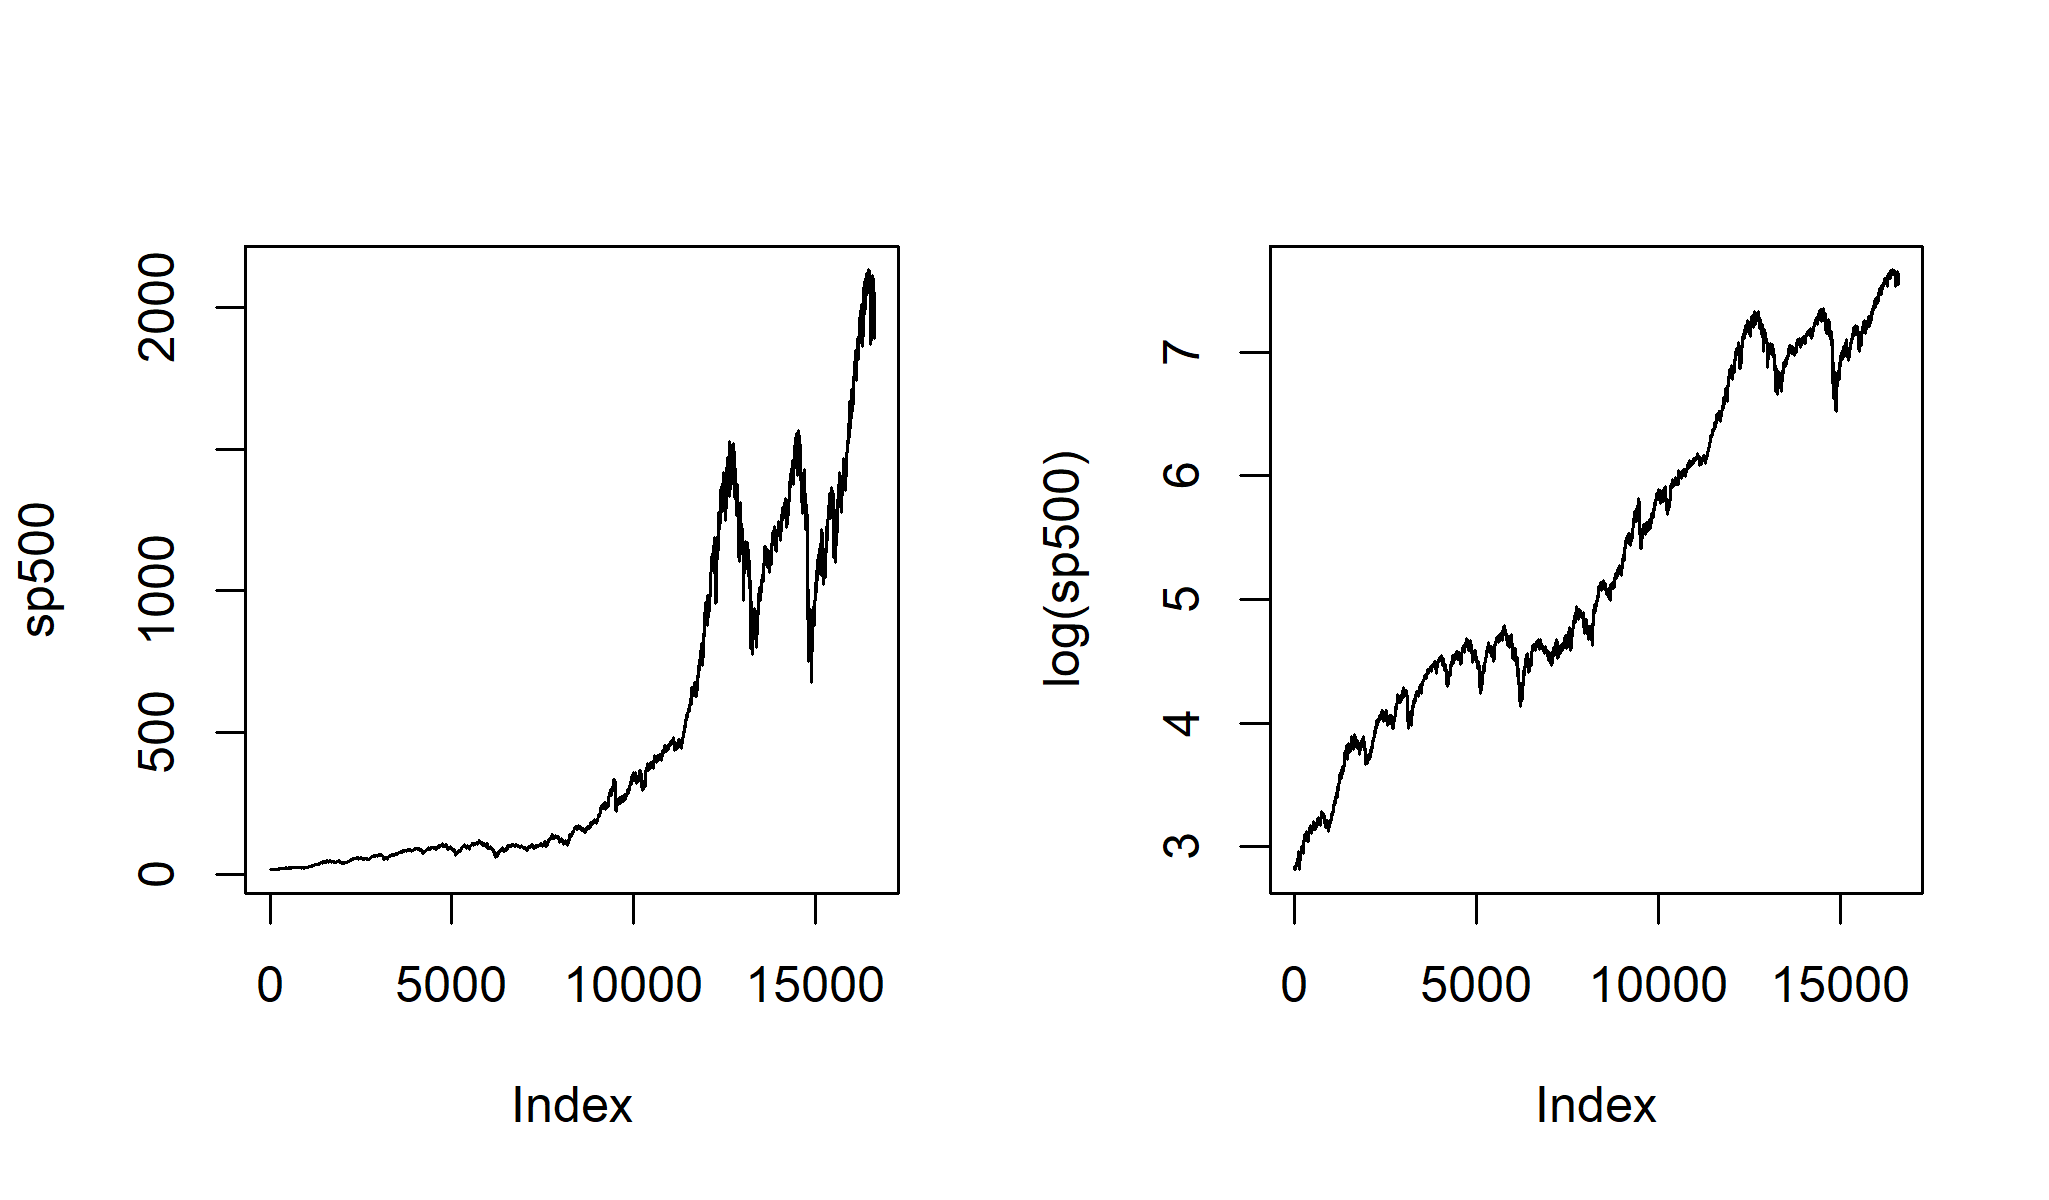
\includegraphics{figure/intro-sp500-1.png}

\begin{itemize}
\tightlist
\item
  To train our intuition, we can compare the data with simulations from
  a fitted model. A simple starting point is a Gaussian random walk with
  drift, having parameters estimated by
\end{itemize}

\begin{Shaded}
\begin{Highlighting}[]
\NormalTok{mu <-}\StringTok{ }\KeywordTok{mean}\NormalTok{(}\KeywordTok{diff}\NormalTok{(}\KeywordTok{log}\NormalTok{(sp500)))}
\NormalTok{sigma <-}\StringTok{ }\KeywordTok{sd}\NormalTok{(}\KeywordTok{diff}\NormalTok{(}\KeywordTok{log}\NormalTok{(sp500)))}
\KeywordTok{set.seed}\NormalTok{(}\DecValTok{95483123}\NormalTok{)}
\NormalTok{X1 <-}\StringTok{ }\KeywordTok{log}\NormalTok{(sp500[}\DecValTok{1}\NormalTok{])}\OperatorTok{+}\KeywordTok{cumsum}\NormalTok{(}\KeywordTok{c}\NormalTok{(}\DecValTok{0}\NormalTok{,}\KeywordTok{rnorm}\NormalTok{(N}\OperatorTok{-}\DecValTok{1}\NormalTok{,}\DataTypeTok{mean=}\NormalTok{mu,}\DataTypeTok{sd=}\NormalTok{sigma)))}
\KeywordTok{set.seed}\NormalTok{(}\DecValTok{324324587}\NormalTok{)}
\NormalTok{X2 <-}\StringTok{ }\KeywordTok{log}\NormalTok{(sp500[}\DecValTok{1}\NormalTok{])}\OperatorTok{+}\KeywordTok{cumsum}\NormalTok{(}\KeywordTok{c}\NormalTok{(}\DecValTok{0}\NormalTok{,}\KeywordTok{rnorm}\NormalTok{(N}\OperatorTok{-}\DecValTok{1}\NormalTok{,}\DataTypeTok{mean=}\NormalTok{mu,}\DataTypeTok{sd=}\NormalTok{sigma)))}
\KeywordTok{par}\NormalTok{(}\DataTypeTok{mfrow=}\KeywordTok{c}\NormalTok{(}\DecValTok{1}\NormalTok{,}\DecValTok{2}\NormalTok{))}
\KeywordTok{plot}\NormalTok{(X1,}\DataTypeTok{type=}\StringTok{"l"}\NormalTok{)}
\KeywordTok{plot}\NormalTok{(X2,}\DataTypeTok{type=}\StringTok{"l"}\NormalTok{)}
\end{Highlighting}
\end{Shaded}
\todo[inline]{Random walk model here only initialized with our first data point (doesn't depend on any others). Here, the drift is estimated using the mean of the cumulative differences}
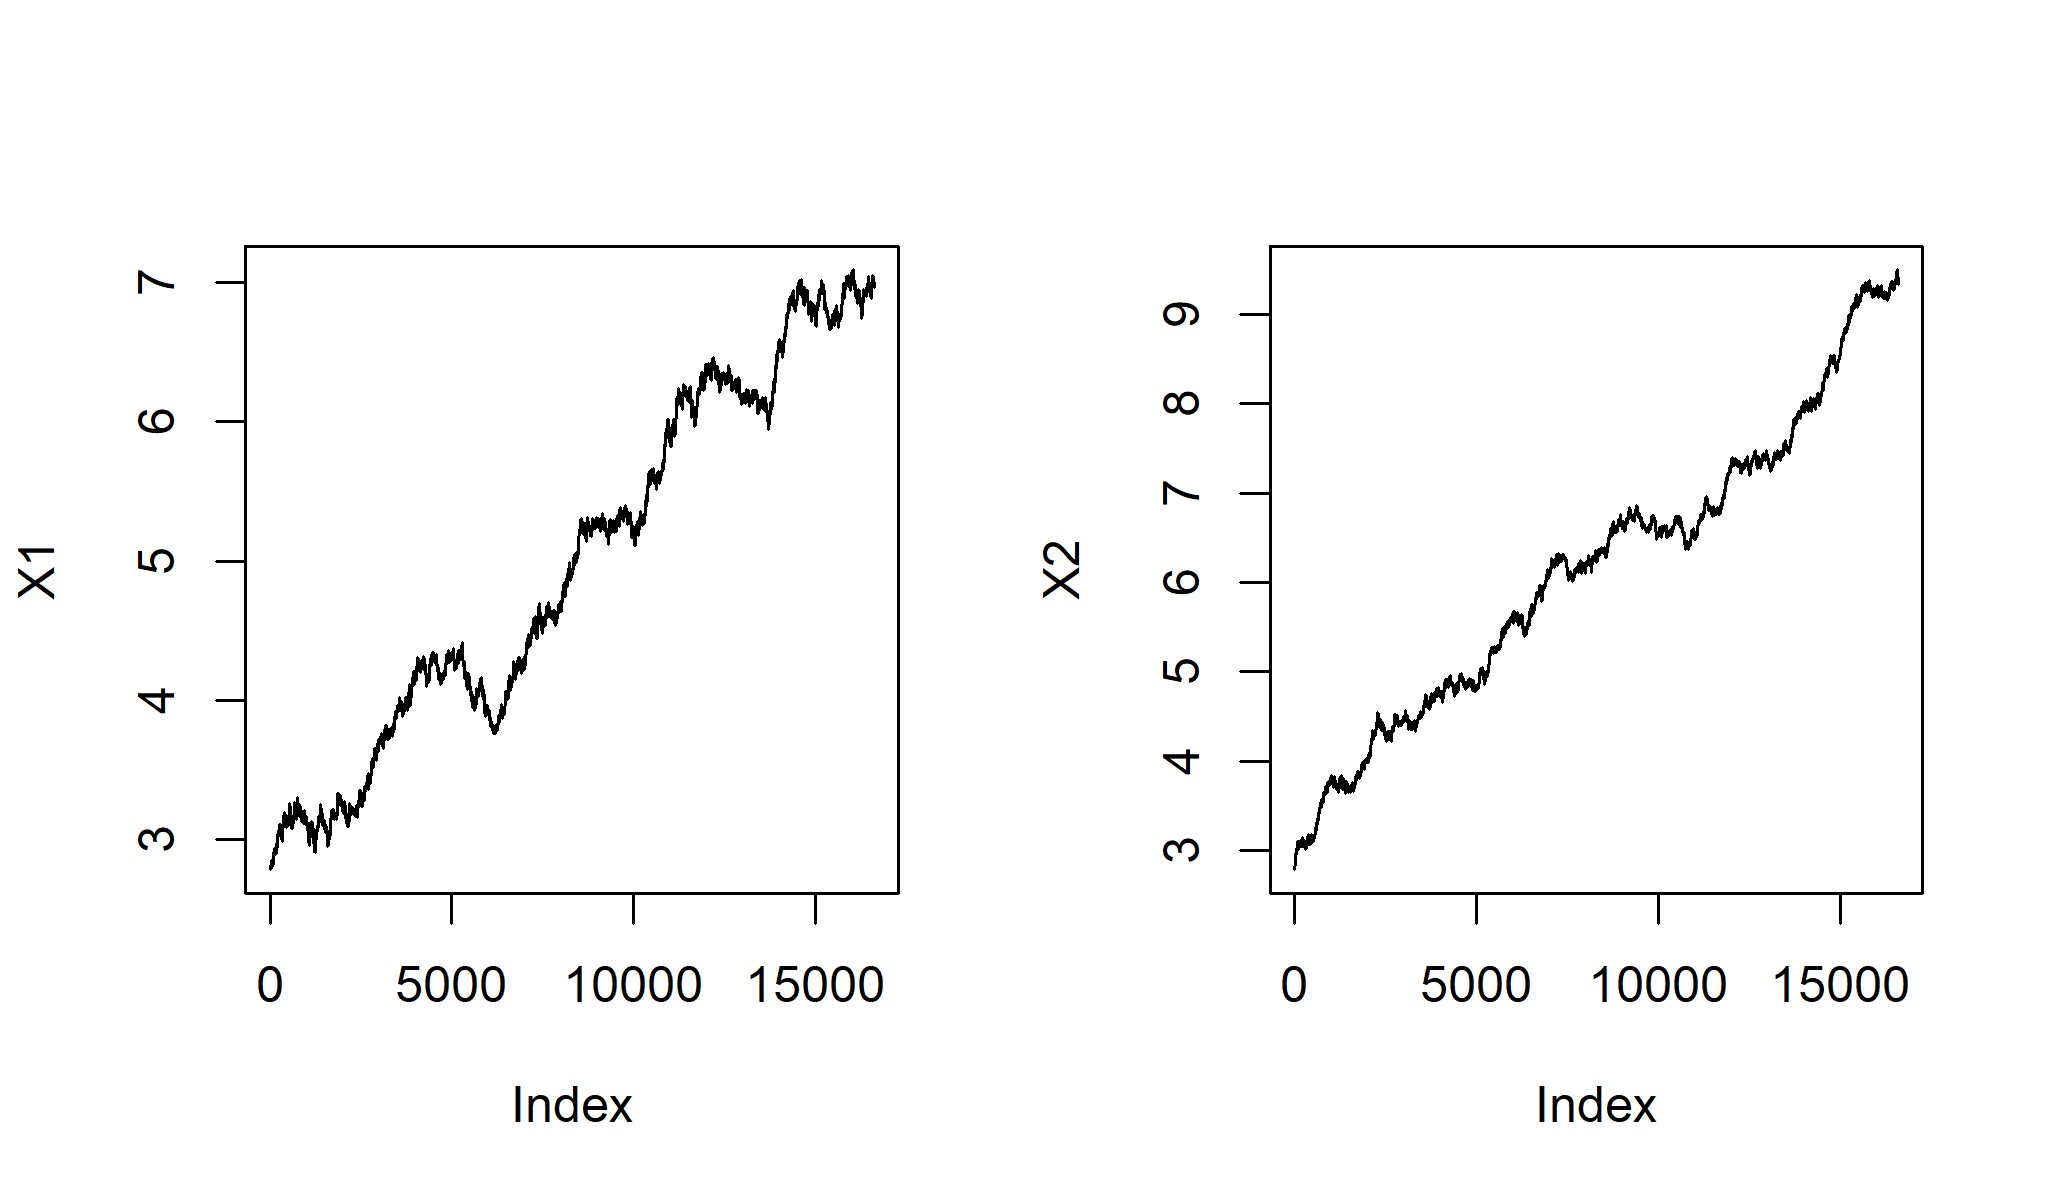
\includegraphics{figure/intro-sp500params-1.png}

\begin{itemize}
\item
  Seems reasonable enough so far. Let's plot the sample autocorrelation
  function (sample ACF) of \texttt{diff(log(sp500))}.
\item
  It is bad style to refer to quantities using computer code notation.
  We should set up mathematical notation in the text. Let's try
  again\ldots{}
\item
  Let \(\data{y_{1:N}}\) be the time series of S\&P 500 daily closing
  values downloaded from yahoo.com. Let
  \(\data{z_n}= \Delta \log \data{y_n} = \log \data{y_{n}}-\log \data{y_{n-1}}\).
\item
  The temporal difference of the log of the value of an investment is
  called the \textbf{return} on the investment. Let's plot the sample
  autocorrelation function of the time series of S\&P 500 returns,
  \(\data{z_{2:N}}\).
\end{itemize}

\begin{Shaded}
\begin{Highlighting}[]
\NormalTok{z <-}\StringTok{ }\KeywordTok{diff}\NormalTok{(}\KeywordTok{log}\NormalTok{(sp500))}
\KeywordTok{acf}\NormalTok{(z)}
\end{Highlighting}
\end{Shaded}

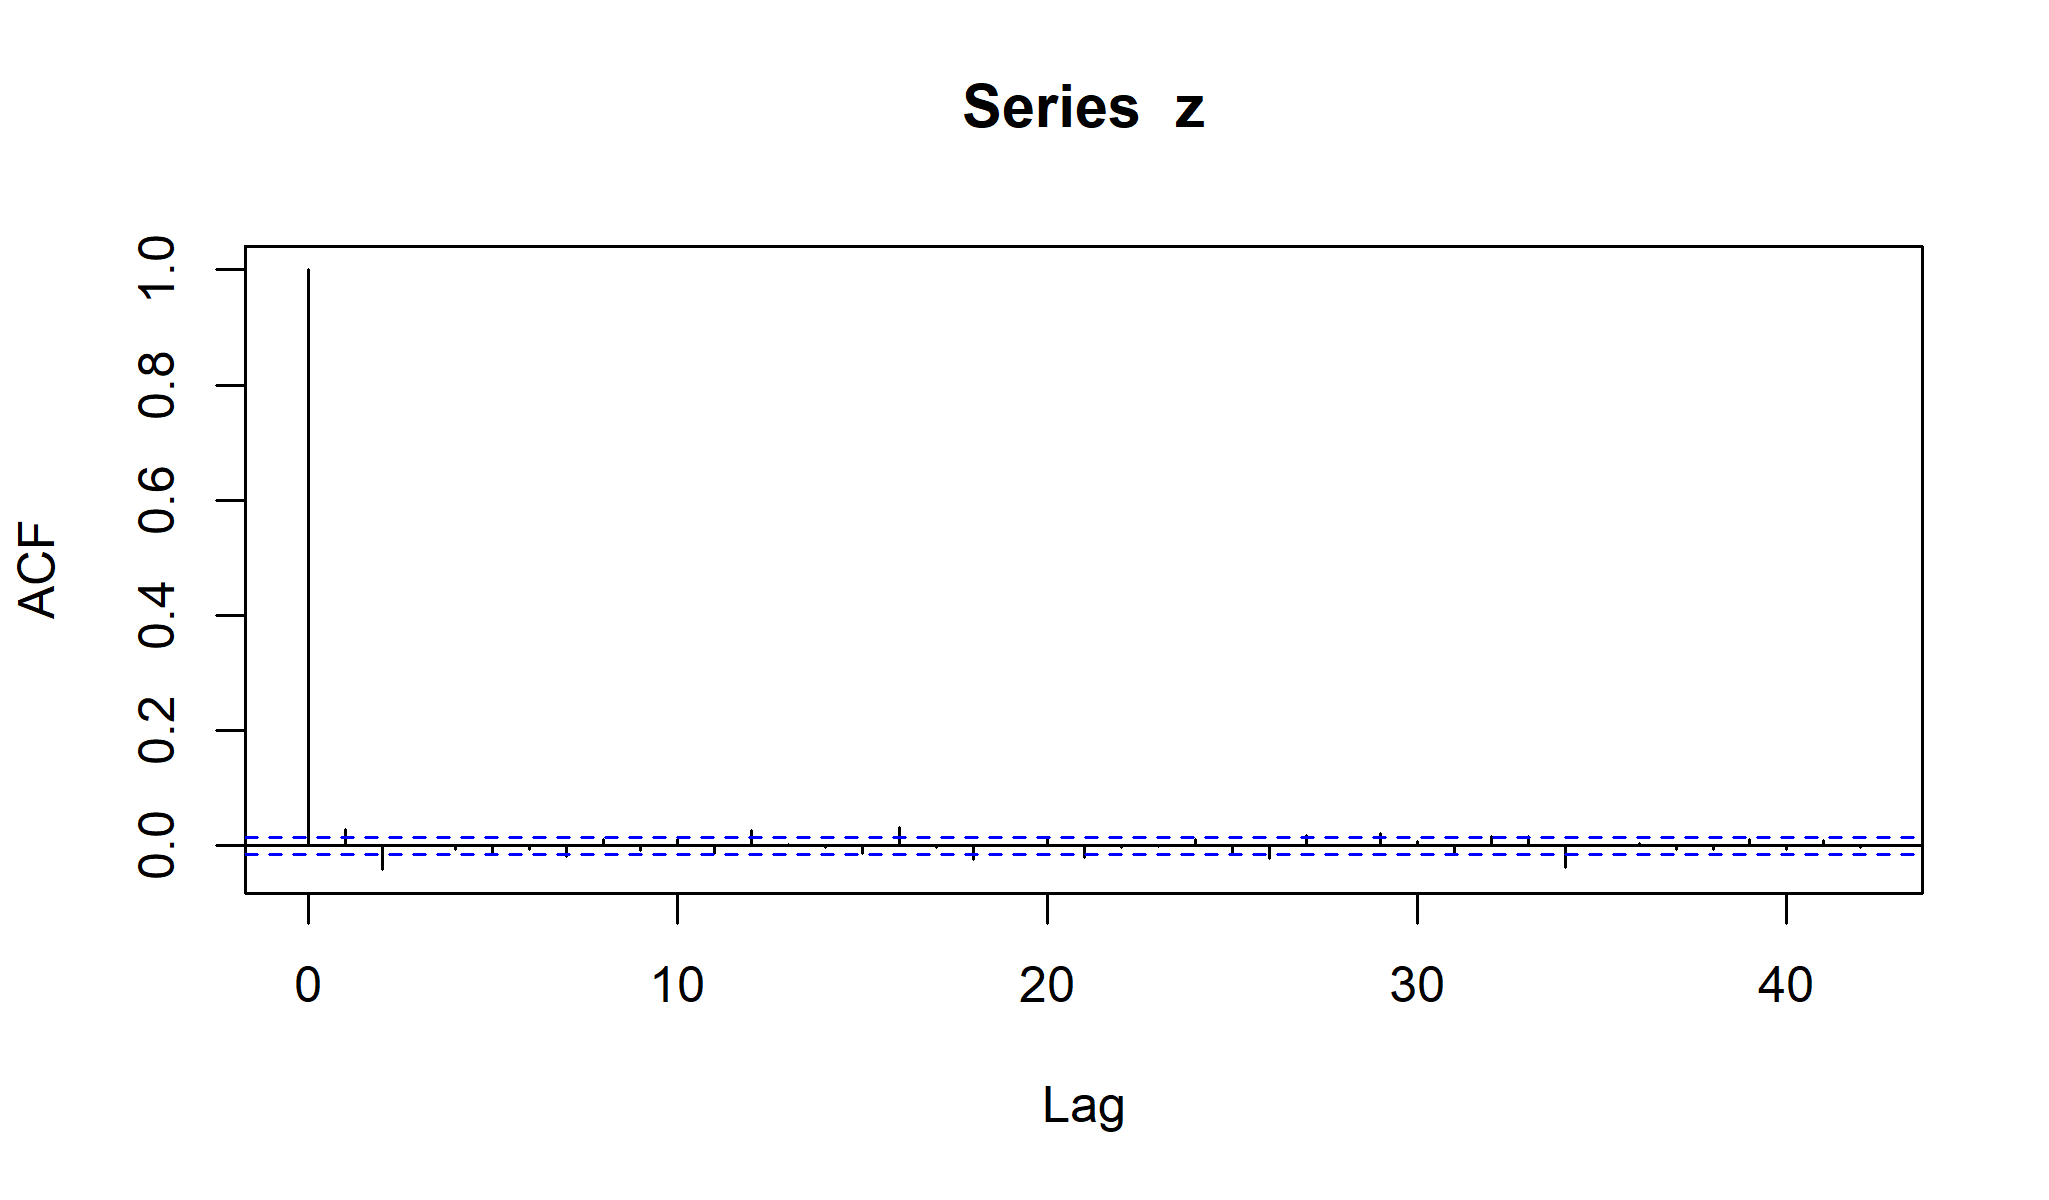
\includegraphics{figure/intro-sp500_acf-1.png}

\begin{itemize}
\item
  This looks pretty close to the ACF of white noise. There is some
  evidence for a small nonzero autocorrelation at lags 0 and 1.
\item
  Here, we have have a long time series (\(N=16616\)). \hl{For such a long
  time series, statistically significant effects may be practically
  insignificant.}
\end{itemize}

\begin{center}\rule{0.5\linewidth}{\linethickness}\end{center}

\begin{center}\rule{0.5\linewidth}{\linethickness}\end{center}

\subsubsection{Question: Why may the length of the time series be
relevant when considering practical versus statistical
significance?}\label{question-why-may-the-length-of-the-time-series-be-relevant-when-considering-practical-versus-statistical-significance}

\begin{center}\rule{0.5\linewidth}{\linethickness}\end{center}

\begin{center}\rule{0.5\linewidth}{\linethickness}\end{center}

\begin{itemize}
\item
  It seems like the S\&P 500 returns (centered, by subtracting the
  sample mean) may be a real-life time series well modeled by white
  noise.
\item
  However, things become less clear when we look at the absolute value
  of the centered returns.
\end{itemize}

\begin{center}\rule{0.5\linewidth}{\linethickness}\end{center}

\begin{center}\rule{0.5\linewidth}{\linethickness}\end{center}

\subsubsection{Question: How should we interpret the following plot? To
what extent does this plot refute the white noise model for the centered
returns (or, equivalently, the random walk model for the log index
value)?}\label{question-how-should-we-interpret-the-following-plot-to-what-extent-does-this-plot-refute-the-white-noise-model-for-the-centered-returns-or-equivalently-the-random-walk-model-for-the-log-index-value}

\begin{Shaded}
\begin{Highlighting}[]
\KeywordTok{acf}\NormalTok{(}\KeywordTok{abs}\NormalTok{(z}\OperatorTok{-}\KeywordTok{mean}\NormalTok{(z)),}\DataTypeTok{lag.max=}\DecValTok{200}\NormalTok{)}
\end{Highlighting}
\end{Shaded}

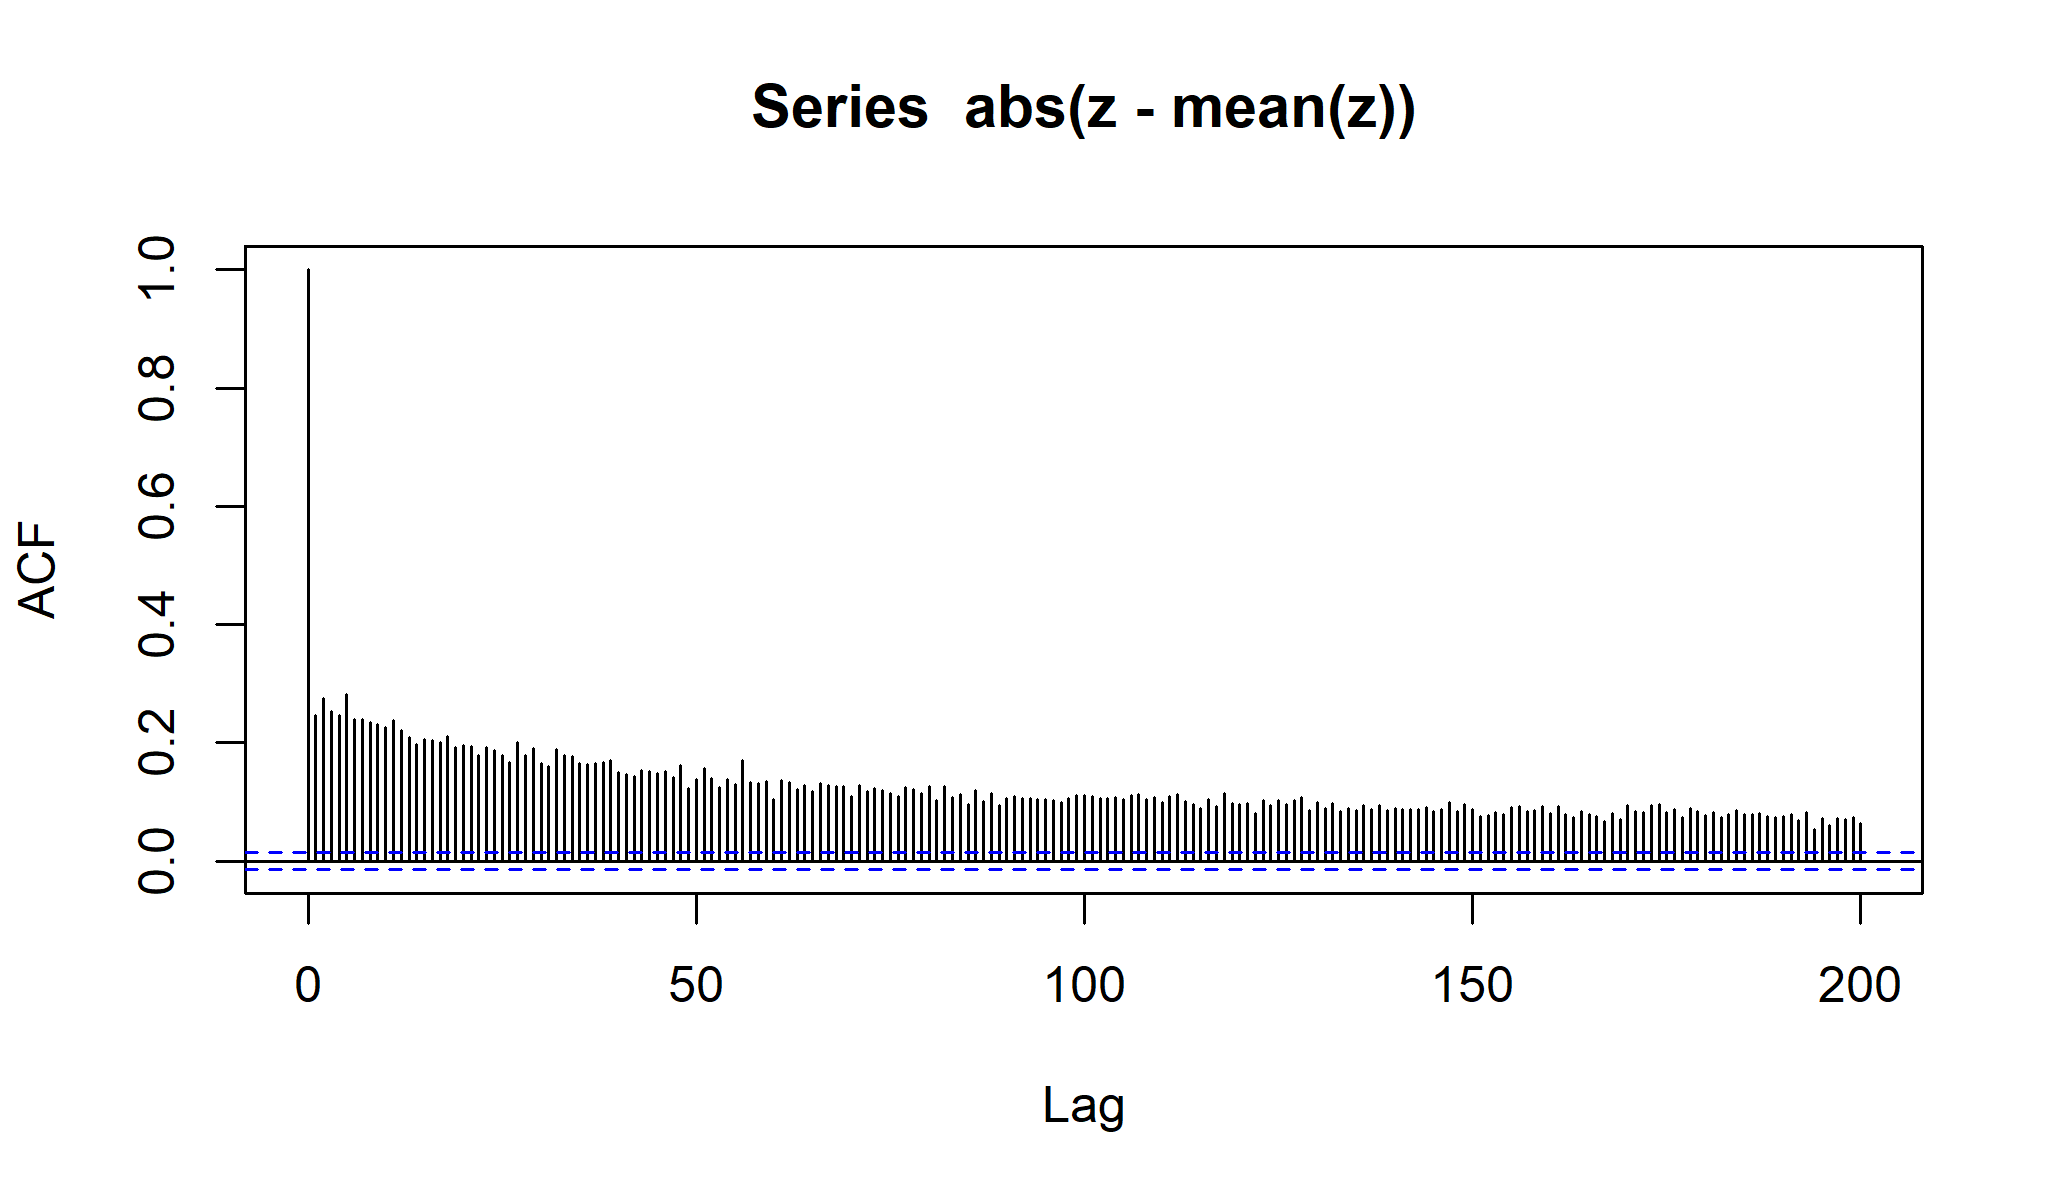
\includegraphics{figure/intro-sp500_abs_return_acf-1.png}

\todo[inline]{Implies that magnitudes are correlated. If a white noise model isn't iid, the correlation in absolute values is possible. But for iid white noise, the absolute values are uncorrelated}

\todo[inline]{Let $\xi_n$ be iid whitenoise. Let $H_n$ be a stationary process independent of $\xi_n$. Claim: $\xi_nH_n$ is white noise with correlated absolute value.}

\begin{center}\rule{0.5\linewidth}{\linethickness}\end{center}

\begin{center}\rule{0.5\linewidth}{\linethickness}\end{center}

\subsubsection{Volatility and market
inefficiencies}\label{volatility-and-market-inefficiencies}

\begin{itemize}
\item
  Nowadays, nobody is surprised that the sample ACF of a financial
  return time series shows little or no evidence for autocorrelation.
\item
  Deviations from the efficient market hypothesis, if you can find them,
  are of interest.
\item
  Also, it remains a challenge to find good models for
  \textbf{volatility}, the conditional variance process of a financial
  return model.
\end{itemize}

\begin{center}\rule{0.5\linewidth}{\linethickness}\end{center}

\begin{center}\rule{0.5\linewidth}{\linethickness}\end{center}


\end{document}
